\documentclass[10pt,twoside]{article}\usepackage[]{graphicx}\usepackage[]{color}
%% maxwidth is the original width if it is less than linewidth
%% otherwise use linewidth (to make sure the graphics do not exceed the margin)
\makeatletter
\def\maxwidth{ %
  \ifdim\Gin@nat@width>\linewidth
    \linewidth
  \else
    \Gin@nat@width
  \fi
}
\makeatother

\definecolor{fgcolor}{rgb}{0.345, 0.345, 0.345}
\newcommand{\hlnum}[1]{\textcolor[rgb]{0.686,0.059,0.569}{#1}}%
\newcommand{\hlstr}[1]{\textcolor[rgb]{0.192,0.494,0.8}{#1}}%
\newcommand{\hlcom}[1]{\textcolor[rgb]{0.678,0.584,0.686}{\textit{#1}}}%
\newcommand{\hlopt}[1]{\textcolor[rgb]{0,0,0}{#1}}%
\newcommand{\hlstd}[1]{\textcolor[rgb]{0.345,0.345,0.345}{#1}}%
\newcommand{\hlkwa}[1]{\textcolor[rgb]{0.161,0.373,0.58}{\textbf{#1}}}%
\newcommand{\hlkwb}[1]{\textcolor[rgb]{0.69,0.353,0.396}{#1}}%
\newcommand{\hlkwc}[1]{\textcolor[rgb]{0.333,0.667,0.333}{#1}}%
\newcommand{\hlkwd}[1]{\textcolor[rgb]{0.737,0.353,0.396}{\textbf{#1}}}%
\let\hlipl\hlkwb

\usepackage{framed}
\makeatletter
\newenvironment{kframe}{%
 \def\at@end@of@kframe{}%
 \ifinner\ifhmode%
  \def\at@end@of@kframe{\end{minipage}}%
  \begin{minipage}{\columnwidth}%
 \fi\fi%
 \def\FrameCommand##1{\hskip\@totalleftmargin \hskip-\fboxsep
 \colorbox{shadecolor}{##1}\hskip-\fboxsep
     % There is no \\@totalrightmargin, so:
     \hskip-\linewidth \hskip-\@totalleftmargin \hskip\columnwidth}%
 \MakeFramed {\advance\hsize-\width
   \@totalleftmargin\z@ \linewidth\hsize
   \@setminipage}}%
 {\par\unskip\endMakeFramed%
 \at@end@of@kframe}
\makeatother

\definecolor{shadecolor}{rgb}{.97, .97, .97}
\definecolor{messagecolor}{rgb}{0, 0, 0}
\definecolor{warningcolor}{rgb}{1, 0, 1}
\definecolor{errorcolor}{rgb}{1, 0, 0}
\newenvironment{knitrout}{}{} % an empty environment to be redefined in TeX

\usepackage{alltt}

\usepackage{suppmat}
\usepackage{listings}
\usepackage[T1]{fontenc} % Better underscores
\usepackage{longtable}
\usepackage{graphicx}

\usepackage[rgb,dvipsnames]{xcolor}
\definecolor{grey}{rgb}{0.5, 0.5, 0.5}

% Enable new column type -- centered with fixed
% Following http://texblog.org/2008/05/07/fwd-equal-cell-width-right-and-centre-aligned-content/
\usepackage{array}
\newcolumntype{x}[1]{%
>{\raggedleft}p{#1}}%

\newcommand{\smurl}[1]{\url{#1}}
\newcommand{\email}[1]{\href{mailto:#1}{\texttt{#1}}}


\title{Is allocation among reproductive tissues coordinated with seed size?}
\runninghead{S\lowercase{hifts in allocation among reproductive tissues}}

\author{E. H. Wenk\textsuperscript{1,\textasteriskcentered}, K. Abramowicz\textsuperscript{2}, D.S. Falster\textsuperscript{1}, M. Westoby\textsuperscript{3} }
\affiliation{
\textsuperscript{1} Evolution and Ecology Research Centre, University of New South Wales, Sydney NSW 2052, Australia \\
\textsuperscript{2} Department of Mathematics and Mathematical Statistics, Ume{\aa} University, 90187 Ume{\aa}, Sweden \\
\textsuperscript{3} Biological Sciences, Macquarie University NSW 2109, Australia \\
\textsuperscript{\textasteriskcentered} Correspondence author. E-mail: \email{ehwenk@gmail.com}
}

\usepackage[authoryear,sectionbib,sort]{natbib}
\bibliographystyle{amnat2}

\pdfminorversion=4
% tell pdflatex to generate PDF in version 1.4
% Needed for problem-free conversion on manuscript central (arrgh)
% http://timotheepoisot.fr/2013/06/24/manuscript-central-pdf-fix/


\titleprefix{Supporting Materials for:}

\date{}



\IfFileExists{upquote.sty}{\usepackage{upquote}}{}
\begin{document}

\maketitle

\begingroup
\let\cleardoublepage\relax
\let\clearpage\relax
\tableofcontents
\endgroup


\renewcommand{\thefigure}{S\arabic{figure}}
\renewcommand{\thetable}{S\arabic{table}}
\setcounter{secnumdepth}{0}


\section{Additional results supporting main text}



\begin{table}[h]
\centering
\caption{Species values for data plotted in Figure 3: shifts in reproductive tissue allocation with seed size.  Counts and costs are per unit leaf area of the plant. The bottom line indicates the corresponding figure of the main text where the data are presented. Data for reproductive costs (Figure 3, panel a), Seed-size, pollen-attraction costs, and provisioning costs (Figure 3, panel f) are presented in Table 1 in the main text and are not included here.}
\label{tab:speciesvals}
{\footnotesize
\begin{tabular}{p{3cm}|p{1cm}p{1cm}|p{1cm}p{1cm}|p{1cm}p{1cm}|p{1cm}p{1cm}|p{1.5cm}p{1cm}}
\hline
& \multicolumn{2}{c|}{} & \multicolumn{2}{c|}{} & \multicolumn{2}{c|}{Proportion} & \multicolumn{2}{c|}{Proportion}& \multicolumn{2}{c}{Proportion} \\
& \multicolumn{2}{c|}{} & \multicolumn{2}{c|}{} & \multicolumn{2}{c|}{pollen-attraction} & \multicolumn{2}{c|}{provisioning}& \multicolumn{2}{c}{success} \\
& \multicolumn{2}{c|}{} & \multicolumn{2}{c|}{} & \multicolumn{2}{c|}{investment to} & \multicolumn{2}{c|}{investment to}& \multicolumn{2}{c}{investment to} \\
% latex table generated in R 3.4.2 by xtable 1.8-2 package
% Wed Feb 14 14:05:36 2018
species & seed count & ovule count & pollen-attraction costs & choosi- ness & success & discarded & success & discarded & pollen-attraction & provi- sioning \\ 
  \hline
\textit{Banksia ericifolia} &  0.01400 &  0.415 & 0.00448 & 123.93 & 0.05634 & 0.944 & 0.873 & 0.127 & 0.00849 & 0.992 \\ 
  \textit{Boronia ledifolia} &  0.33953 & 11.025 & 0.11353 &  68.63 & 0.06853 & 0.931 & 0.572 & 0.428 & 0.21759 & 0.782 \\ 
  \textit{Conospermum ericifolium} &  0.46255 &  2.845 & 0.08337 &   7.14 & 0.18011 & 0.820 & 0.306 & 0.694 & 0.40425 & 0.596 \\ 
  \textit{Epacris microphylla} & 19.66781 & 74.846 & 0.00318 &   6.37 & 0.35841 & 0.642 & 0.329 & 0.671 & 0.81629 & 0.184 \\ 
  \textit{Grevillea buxifolia} &  0.01083 &  0.820 & 0.02654 &  83.99 & 0.02214 & 0.978 & 0.671 & 0.329 & 0.06174 & 0.938 \\ 
  \textit{Grevillea speciosa} &  0.01010 &  0.940 & 0.01372 & 210.93 & 0.03085 & 0.969 & 0.504 & 0.496 & 0.07767 & 0.922 \\ 
  \textit{Hakea teretifolia} &  0.00245 &  0.590 & 0.00647 & 355.20 & 0.00468 & 0.995 & 0.517 & 0.483 & 0.05648 & 0.944 \\ 
  \textit{Hemigenia purpurea} &  1.47663 &  5.674 & 0.07291 &   4.68 & 0.33126 & 0.669 & 0.380 & 0.620 & 0.56216 & 0.438 \\ 
  \textit{Leucopogon esquamatus} &  0.70031 &  2.241 & 0.04240 &   8.00 & 0.32664 & 0.673 & 0.544 & 0.456 & 0.28809 & 0.712 \\ 
  \textit{Persoonia lanceolata} &  0.01030 &  0.128 & 0.02313 &  37.64 & 0.06294 & 0.937 & 0.710 & 0.290 & 0.06415 & 0.936 \\ 
  \textit{Petrophile pulchella} &  0.19390 &  0.556 & 0.07134 &   5.02 & 0.33887 & 0.661 & 0.856 & 0.144 & 0.11287 & 0.887 \\ 
  \textit{Phyllota phylicoides} &  0.04014 &  0.923 & 0.02351 &  82.84 & 0.04775 & 0.952 & 0.453 & 0.547 & 0.47996 & 0.520 \\ 
  \textit{Pimelea linifolia} &  1.23518 &  4.514 & 0.22509 &   4.36 & 0.27360 & 0.726 & 0.818 & 0.182 & 0.70018 & 0.300 \\ 
  \textit{Pultenaea tuberculata} &  0.04731 &  0.789 & 0.04729 &  26.12 & 0.06759 & 0.932 & 0.421 & 0.579 & 0.62784 & 0.372 \\ 
   \hline
Figure reference & \multicolumn{2}{c|}{Fig. 3, panel a} & \multicolumn{2}{c|}{Fig. 3, panel b} & \multicolumn{2}{c|}{Fig. 3, panel c} & \multicolumn{2}{c|}{Fig. 3, panel d}  & \multicolumn{2}{c}{Fig. 3, panel e}\\
\hline
\end{tabular}
}
\end{table}

\clearpage

\begin{figure}[h]
\centering
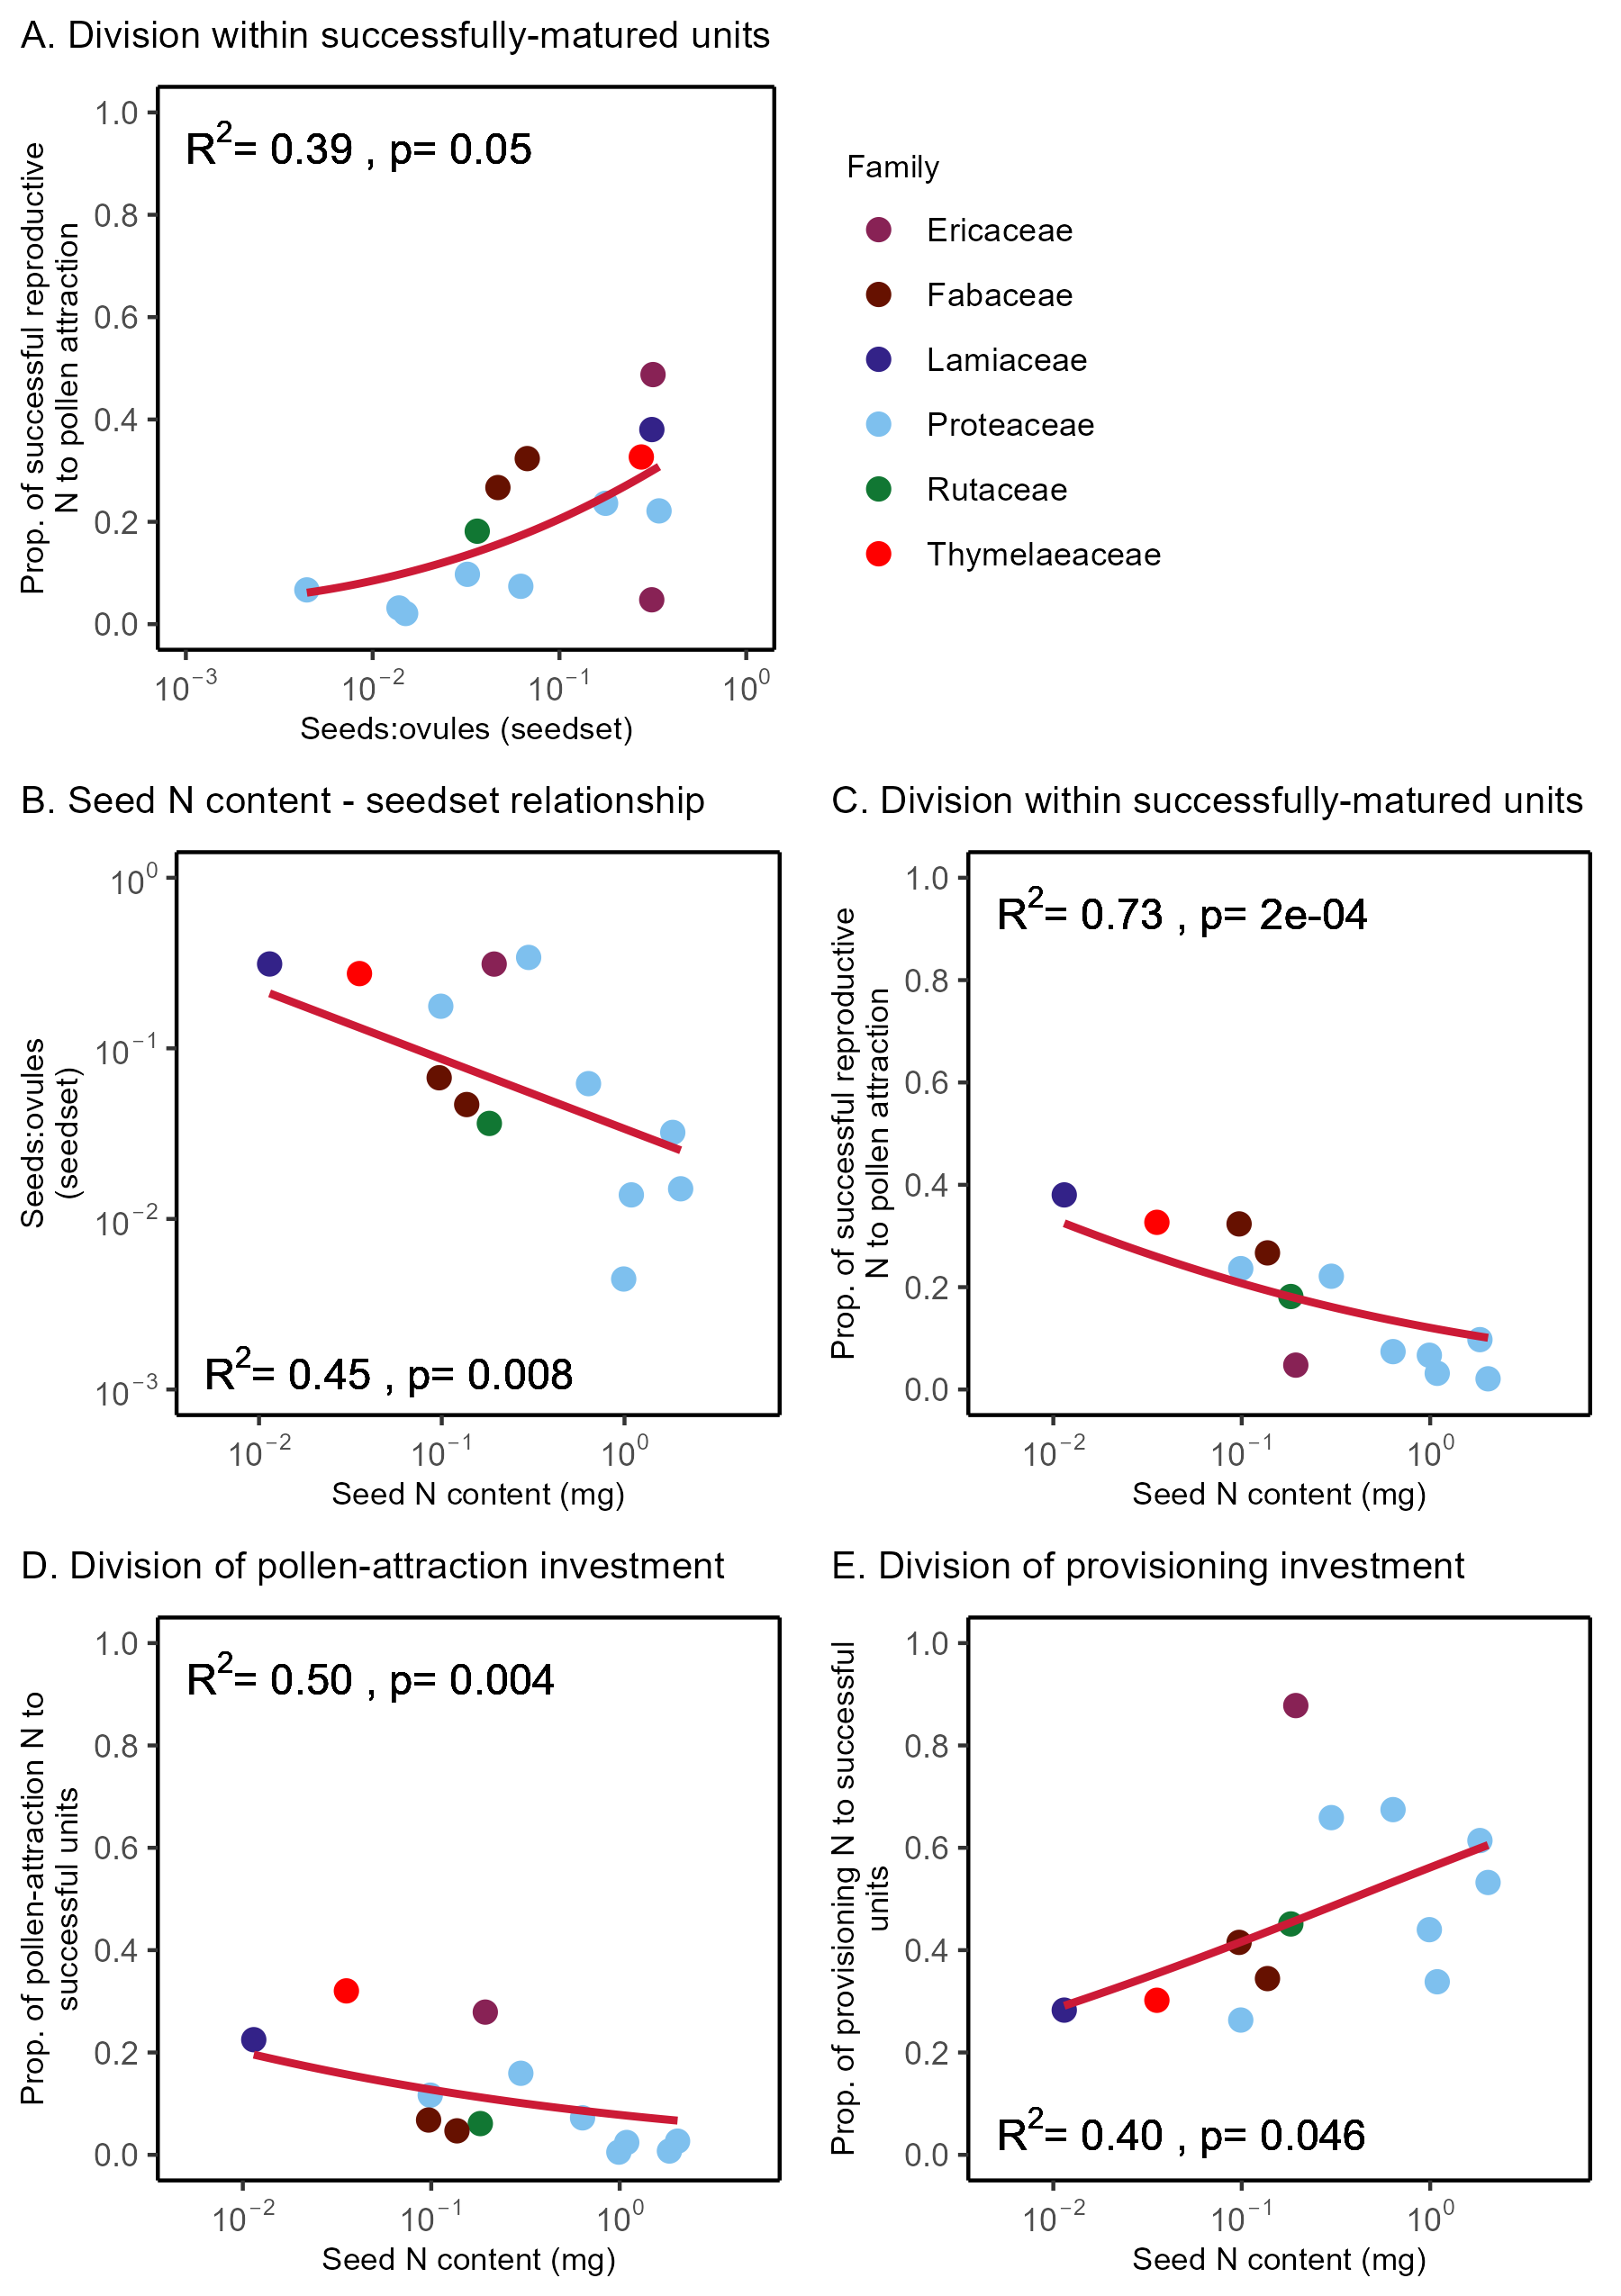
\includegraphics[width=12cm]{Figure3N.png}
\caption{Correlations depicted in Figure 3, using nitrogen content instead of biomass. A) Proportion of successful nitrogen investment going to pollen attraction rather than to seed provisioning (the parental optimist-pessimist spectrum) in relation to seed set (seed to ovule ratio); B) Seed set in relation to seed nitrogen content; C) Proportion successful nitrogen investment to pollen attraction tissues (versus to seed provisioning) in relation to seed nitrogen content; D) Proportion of pollen-attraction nitrogen investment to successful (versus discarded) tissues in relation to seed nitrogen content; and E) Proportion of provisioning nitrogen investment to successful (versus discarded) tissues in relation to seed nitrogen content. Note the log-scale axes for all variables that are not proportions. Lines are fitted using a generalised linear model, using logit link when the outcome is a proportion (bounded from 0-1). The logit link accounts for non-linear shape of relationships. Insets show the proportion of variance explained and p-value.}
\end{figure}

\clearpage

\begin{figure}[h]
  \centering
  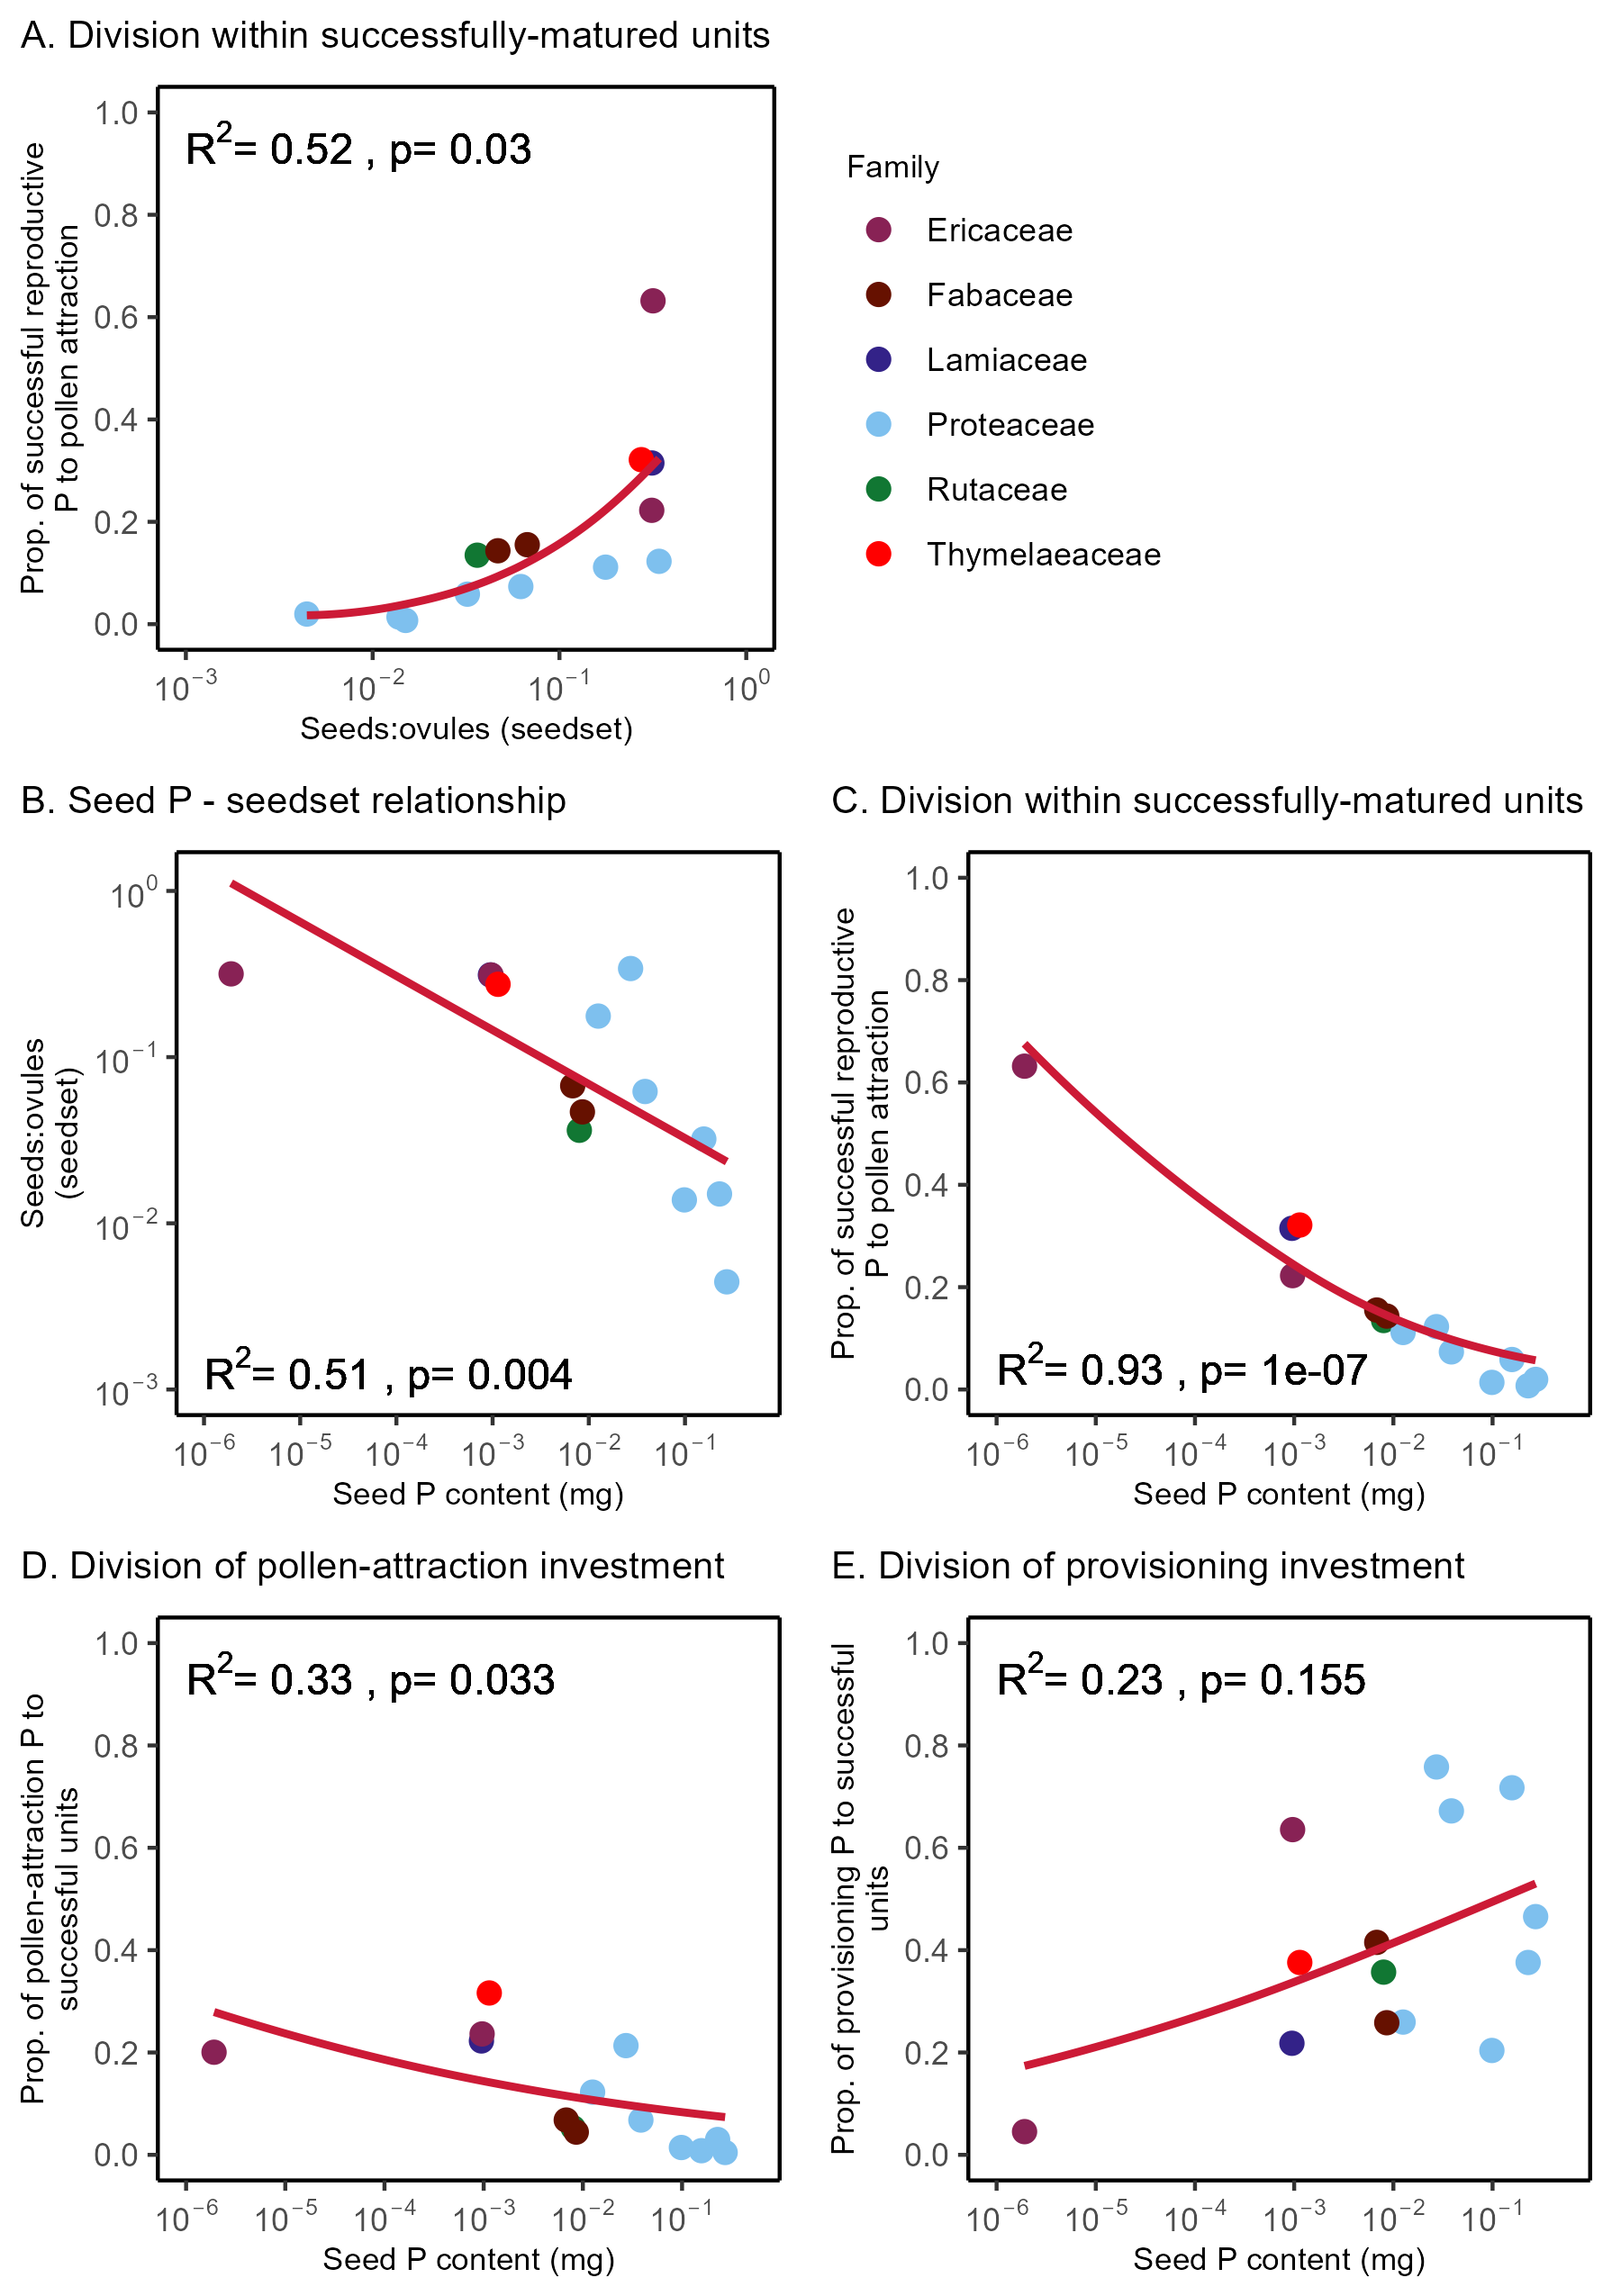
\includegraphics[width=12cm]{Figure3P.png}
  \caption{Correlations depicted in Figure 3, using phosphorus content instead of biomass. A) Proportion of successful phosphorus investment going to pollen attraction rather than to seed provisioning (the parental optimist-pessimist spectrum) in relation to seed set (seed to ovule ratio); B) Seed set in relation to seed phosphorus content; C) Proportion successful phosphorus investment to pollen attraction tissues (versus to seed provisioning) in relation to seed phosphorus content; D) Proportion of pollen-attraction phosphorus investment to successful (versus discarded) tissues in relation to seed phosphorus content; and E) Proportion of provisioning phosphorus investment to successful (versus discarded) tissues in relation to seed phosphorus content. Note the log-scale axes for all variables that are not proportions. Lines are fitted using a generalised linear model, using logit link when the outcome is a proportion (bounded from 0-1). The logit link accounts for non-linear shape of relationships. Insets show the proportion of variance explained and p-value.}
  \end{figure}
  
\clearpage

\begin{table}[h]
\centering
\caption{Intraspecific correlations between total reproductive investment and (a) propagule investment and (b) flower investment, where flower investment is defined as 'flower weight $\times$ bud count'. Due to the high proportion of aborted flowers, flower investment was a better proxy of reproductive investment than was propagule investment. This was true both across species (Figure 5, Table 2 in the main text) and within species, as is shown here.}
\label{tab:propagule_invest_vs_repro}
\begin{tabular}{p{4cm}|x{.75cm}x{1cm}x{1.5cm}|x{.75cm}x{1cm}p{1.5cm}}
\hline
& \multicolumn{3}{c|}{Total reproductive investment} & \multicolumn{3}{c}{Total reproductive investment} \\
& \multicolumn{3}{c|}{vs. propagule investment} & \multicolumn{3}{c}{vs. flower investment} \\
% latex table generated in R 3.4.2 by xtable 1.8-2 package
% Wed Feb 14 14:05:40 2018
Species & n & r$^2$ & p & n & r$^2$ & p \\ 
  \hline
\textit{Banksia ericifolia} &  6 & 0.85 & 0.009 &  6 & 0.92 & 0.002 \\ 
  \textit{Boronia ledifolia} & 24 & 0.53 & < 0.001 & 24 & 0.95 & < 0.001 \\ 
  \textit{Conospermum ericifolium} & 14 & 0.89 & < 0.001 & 14 & 0.87 & < 0.001 \\ 
  \textit{Epacris microphylla} & 28 & 0.74 & < 0.001 & 28 & 0.97 & < 0.001 \\ 
  \textit{Grevillea buxifolia} & 12 & 0.51 & 0.01 & 12 & 0.97 & < 0.001 \\ 
  \textit{Grevillea speciosa} & 12 & 0.55 & 0.006 & 12 & 0.56 & 0.005 \\ 
  \textit{Hakea teretifolia} & 12 & 0.77 & < 0.001 & 12 & 0.89 & < 0.001 \\ 
  \textit{Hemigenia purpurea} & 17 & 0.70 & < 0.001 & 17 & 0.92 & < 0.001 \\ 
  \textit{Leucopogon esquamatus} & 23 & 0.71 & < 0.001 & 23 & 0.99 & < 0.001 \\ 
  \textit{Persoonia lanceolata} &  6 & 0.84 & 0.01 &  6 & 0.92 & 0.002 \\ 
  \textit{Petrophile pulchella} &  9 & 0.30 & 0.129 &  9 & 0.98 & < 0.001 \\ 
  \textit{Phyllota phylicoides} & 19 & 0.32 & 0.012 & 19 & 0.99 & < 0.001 \\ 
  \textit{Pimelea linifolia} & 13 & 0.78 & < 0.001 & 13 & 0.99 & < 0.001 \\ 
  \textit{Pultenaea tuberculata} & 28 & 0.49 & < 0.001 & 28 & 0.99 & < 0.001 \\ 
   \hline

\end{tabular}
\end{table}

\clearpage


\section{Additional details on methods}

\subsection{Methods for calculating nutrient content of reproductive tissues}

Nutrient contents were measured on a selection of reproductive tissues for each species, with 2 – 4 replicates collected across sites. Nutrient contents were independently measured for flowers (including buds), green floral parts (bracts, calyces), immature fruits, mature fruits/seeds/propagules (depending on species), and woody cones, with additional subdivisions of tissues for some taxa.  For some reproductive tissues and for senesced leaves for some species, samples were bulked from many individuals to achieve a sufficiently large sample size. Tissue nitrogen content was determined by combustion using a LECO TruSpec CHN analyser. For phosphorus determination, tissue samples were digested in acid and total P concentration determined by inductively coupled plasma optical emission spectrometry (ICP-OES).  

\subsection{Methods for calculating investment in reproductive tissues}

We collected data for 14 species (Table \ref{tab:species}) at 7 sites (Tables \ref{tab:sites}, Fig. \ref{fig:map}). Individuals were selected as described in the main text.

% latex table generated in R 3.4.2 by xtable 1.8-2 package
% Wed Feb 14 14:05:40 2018
\begingroup\small
\begin{longtable}{p{5cm}p{3cm}p{5cm}p{2cm}}
\caption{Details on study species.} \\ 
  \hline
Scientific name & Family & Common name & Abbreviation \\ 
  \hline
Banksia ericifolia & Proteaceae & Heath banksia & BAER \\ 
  Boronia ledifolia & Rutaceae & Sydney boronia & BOLE \\ 
  Conospermum ericifolium & Proteaceae & Coneseeds & COER \\ 
  Epacris microphylla & Ericaceae & Coast coral heath & EPMI \\ 
  Grevillea buxifolia & Proteaceae & Grey spider flower & GRBU \\ 
  Grevillea speciosa & Proteaceae & Red spider flower & GRSP \\ 
  Hakea teretifolia & Proteaceae & Needlebush; dagger hakea & HATE \\ 
  Hemigenia purpurea  & Lamiaceae & Common hemigenia & HEPU \\ 
  Leucopogon esquamatus & Ericaceae & Swamp beard heath & LEES \\ 
  Persoonia lanceolata & Proteaceae & Lance-leaf geebung & PELA \\ 
  Petrophile pulchella & Proteaceae & Common conesticks & PEPU \\ 
  Phyllota phylicoides & Fabaceae & Heath phyllota & PHPH \\ 
  Pimelea linifolia & Thymelaeaceae & Slender rice flower & PILI \\ 
  Pultenaea tuberculata (previously Pultenaea elliptica) & Fabaceae & Wreath bush-pea & PUTU \\ 
   \hline
\hline
\label{tab:species}
\end{longtable}
\endgroup
% latex table generated in R 3.4.2 by xtable 1.8-2 package
% Wed Feb 14 14:05:40 2018
\begingroup\small
\begin{longtable}{p{2cm}p{1cm}p{1cm}p{1cm}p{1.2cm}p{1.2cm}p{1.2cm}p{1.2cm}p{5cm}}
\caption{Details on study sites.} \\ 
  \hline
Site & Date of fire & Age at harvest & UTM zone & UTM easting & UTM northing & Longitude & Latitude & Notes \\ 
  \hline
Wilunga2012 & 2013 & 1.35 & 56 & 338791 & 6278908 & 151.2622 & -33.6174 &  \\ 
  Waratah2011 & 2011 & 2.40 & 56 & 338404 & 6276308 & 151.2575 & -33.6408 & two cohorts of individuals followed at this site with ages of 1.4 and 2.4 yrs at harvest \\ 
  Basin2007 & 2007 & 5.00 & 56 & 340916 & 6281422 & 151.2855 & -33.5951 & this site is excluded from some fits - although the plants here display RA patterns consistent with other sites, their actual growth is quite stunted in comparison to other similar aged sites \\ 
  Basin2005 & 2005 & 7.00 & 56 & 340734 & 6281614 & 151.2836 & -33.5933 &  \\ 
  Waratah2003 & 2003 & 9.00 & 56 & 338359 & 6276250 & 151.2570 & -33.6413 & part of site burnt in late winter 2015 \\ 
  Basin1981 & 1981 & 32.00 & 56 & 340886 & 6281385 & 151.2852 & -33.5954 & most of site burnt in autumn 2016 \\ 
   \hline
\hline
\label{tab:sites}
\end{longtable}
\endgroup


\begin{figure}[h]
\centering
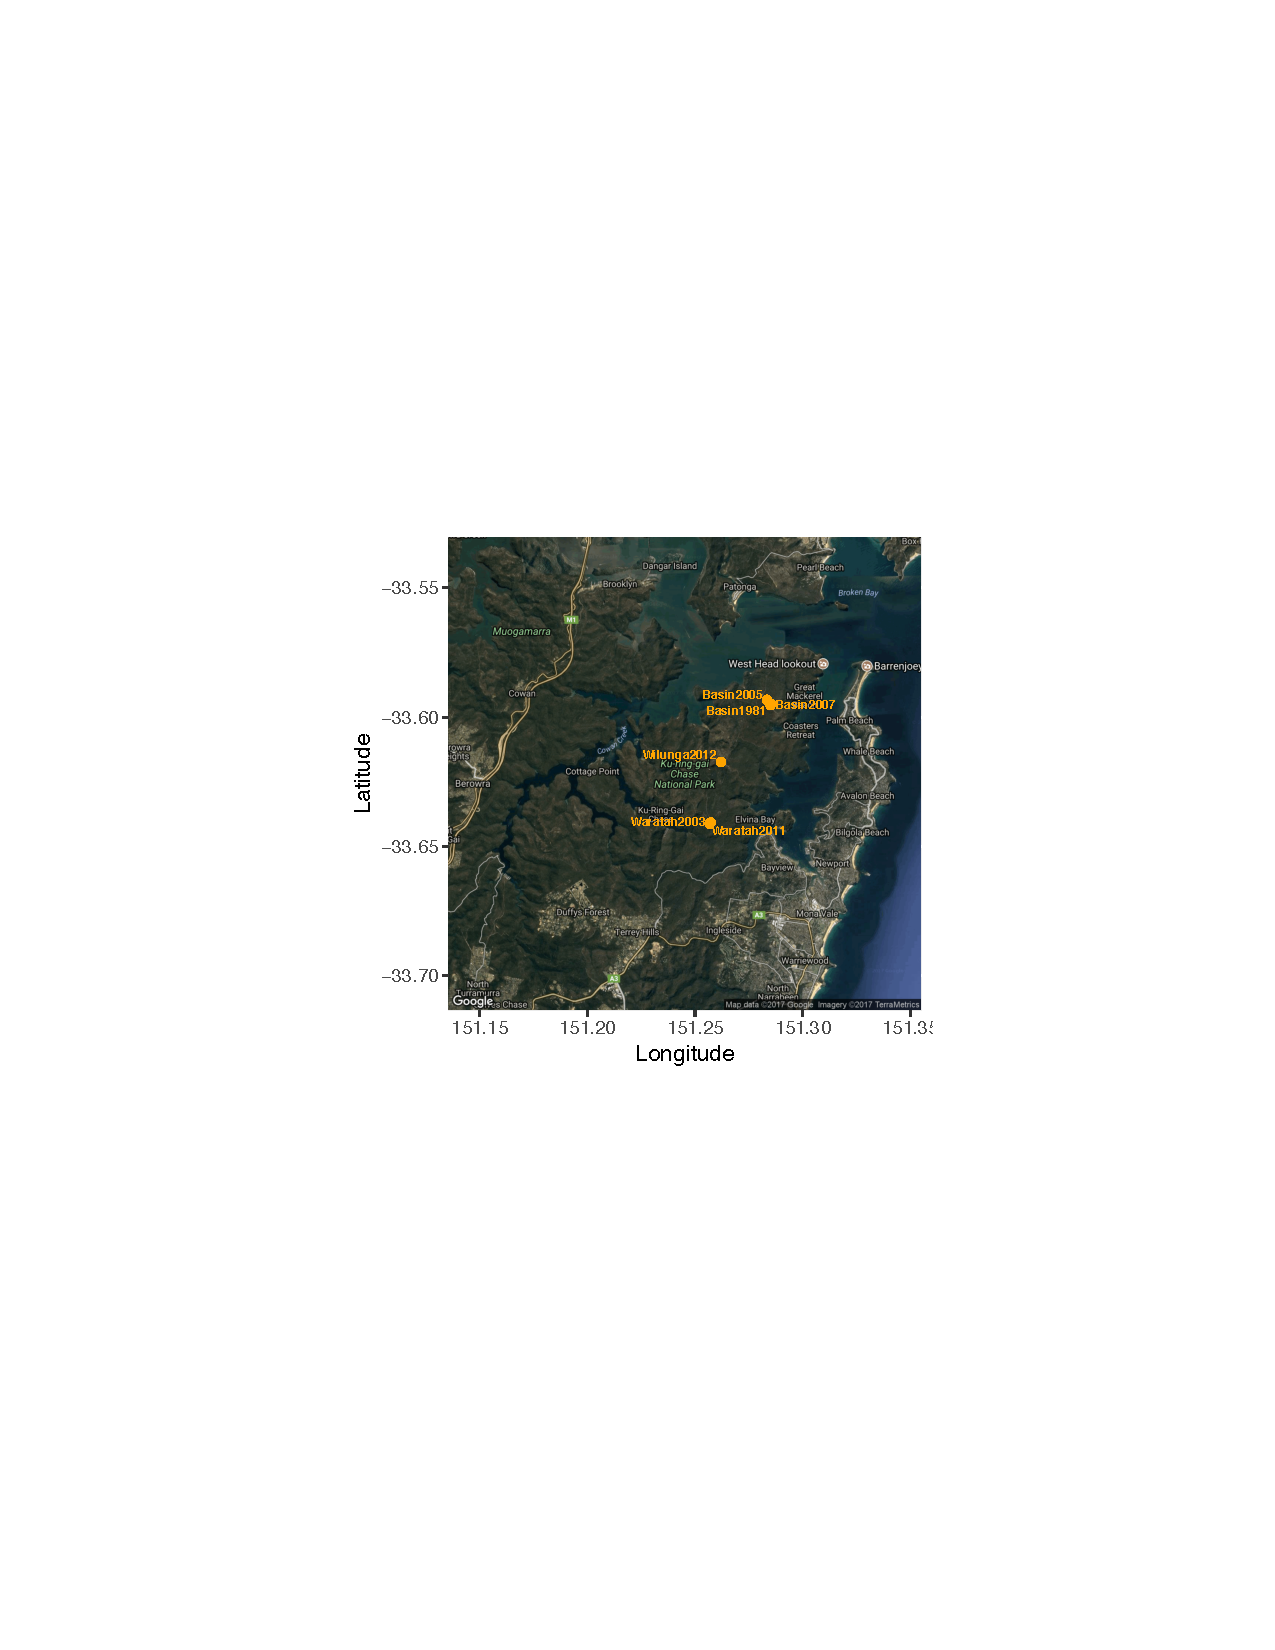
\includegraphics[]{../map.pdf}
\caption{Map of study locations.}
\label{fig:map}
\end{figure}
\clearpage

\begin{figure}[h]
\centering
\includegraphics[]{../phylogeny.pdf}
\caption{Phylogeny of study species, usng V.PhyloMaker2 (Jin and Qian 2022)}
\label{fig:phylogeny}
\end{figure}
\clearpage


For each species, we established a list of different reproductive tissue parts and mapped how these parts developed through time. In all species, reproductive tissue development initiates with a bud or inflorescence bud, which increases in size and is divided into multiple tissue types several times during development. For instance, a bud, once open, divides into being petals + stamens, a sepal, and a stigma. As a pollinated stigma develops into a fruit, it will be further divided into seed, seed pod, and potentially additional parts. The central development axis terminates with the formation of a mature seed, while side axes end in fully developed tissues (such as petals, calyx, pedicel) and aborted tissues (aborted seeds, aborted fruit) at the point where they cease to increase in mass.

While all species developed reproductive tissues from buds to seeds, species showed different developmental pathways due to the precise reproductive tissues used. We therefore created a developmental flowchart for each species, as shown below in following sections in Figs. \ref{fig:map_Banksia_ericifolia}-\ref{fig:map_Pultenaea_tuberculata}). Tables \ref{tab:parts_Banksia_ericifolia}-Table \ref{tab:parts_Pultenaea_tuberculata} then provide, for each species, a list of plant parts, a description of exactly what tissues are included in each plant part and at what developmental stage, the method whereby the count and mass of the plant parts is measured, and the number of ovules in each unit of plant part.

\subsubsection{How the census is completed for each part}

The count of each reproductive tissue type was determined for each individual at each census time. For some reproductive parts a simple count is practical, while for species with a large number of buds (or flowers or fruit) that are regularly spaced along branches, the length of stem covered in buds is a better measure. These lengths were converted into counts through a species-level estimate of "flowers per length". For species that form cones, the cones can be notably different in size and each cone's dimensions was recorded throughout development. The counts of flowers (or other reproductive tissues) were then converted to a count of ovules using the values in the variable \texttt{Multiplier per factor}. Tables \ref{tab:parts_Banksia_ericifolia}-Table \ref{tab:parts_Pultenaea_tuberculata} indicate for each species and plant part, the method used to estimate the mass of parts.


\subsubsection{How parts weights are determined}

For all plant parts, a sample of the representative part was collected from other individuals growing nearby the sample population. We then estimated an average mass of that tissue part for each species. For plant parts that vary considerably in size, such as cones, the mass of parts of different sizes were measured and a regression of mass per length or mass per volume was established. For some individuals, actual reproductive parts were collected. This includes any reproductive parts of the plants at the time of harvest. In addition, some seeds were collected once mature, but before they were dispersed. Whenever actual reproductive parts were collected from an individual, the unit mass of these structures was used instead of the population mean. The data are tabulated in the file flowerParts.csv within the data folder of the project's public GitHub repository (https://github.com/traitecoevo/reproductive_allocation_kuringgai/).

\subsubsection{How investment in each part is estimated}


Our goal was to estimate the amount of mass each plant invests in different tissues within each census period from field data recording the numbers of each part type at successive census dates for a given plant. To achieve this we apply an accounting algorithm to estimate the number of units that have progressed from one category to another in the interval between censuses. The algorithm works as follows:

\begin{itemize}
\item At each census, we compare the number of each part with possible numbers of predecessors from the prior census. Predecessors are those parts that lie at the same or younger age in the plant maps.
\item For a each part in turn, we try to identify the most obvious predecessor, being the one with minimal amount of progression needed to satisfy successive censuses. The predecessor is removed from the list of possible predecessors and the process sis repeated until all parts have predecessors.
\item After finding a predecessor, the investment needed to progress  is calculated. The investment is defined as the difference between the element mass at the time of census and that of it's predecessor.
\end{itemize}

As an example, if, in census $t$, a large bud exists, it is assumed that it has developped from a medium sized bud (the previous stage) in census $t$-1. If in census $t$-1 no medium buds exists, the large bud is assumed to have developped from a small bud (two stages back). This process continues back along the plant map developmental trajectory until a plausible predecessor is located in the previous census period. After this process is complete, any parts from census $t$-1 for which a subsequent developmental stage is not identified as designated as having reached their final developmental stage at census $t$-1 (i.e. they aborted). For plant parts, such as petals, that is a final development stage, no success is sought.


\subsection{Details on calculations by species}

The algorithm for estimating reproductive investment is adjusted for each species according to the specific developmental pathway it uses to produce seeds. Below, for each species we provide a graphic illustration of the pathway used (Figs. \ref{fig:map_Banksia_ericifolia}-\ref{fig:map_Pultenaea_tuberculata}), and tables detailing specific about each part (Tables \ref{tab:parts_Banksia_ericifolia}-Table \ref{tab:parts_Pultenaea_tuberculata}).  Figure \ref{fig:map_key} provides a key on the colouring in Figs. \ref{fig:map_Banksia_ericifolia}-\ref{fig:map_Pultenaea_tuberculata}).

Each plant map begins with a bud (or the appropriate starting point for reproductive tissue development for a specific species) and depicts graphically how the tissue develops through the plant's reproductive cycle to a seed or mature fruit. During the reproductive cycle, there will be branches off the central tissue axis (development from bud to seed). Some of these lead to aborted tissue types (colored red in the graph maps below) and others lead to tissues that reach their final development stage and are then shed by a plant (e.g. petals, calyx, seed pod; colored green in the graph maps below). For some species, there are multiple axes of development. For instance, cones and flowers on a cone have separate axes, because the number of flowers on a cone is inconsistent across individuals. A few species have aborted plant parts that are listed as a separate axis. In these cases, the aborted unit weighs less than a bud and therefore cannot be shown as ever having reached the stage of a bud.

\begin{figure}[h]
\centering
\includegraphics[width=]{../plant_maps/crop/key.png}
\caption{Key describing use of colour in Figs. \ref{fig:map_Banksia_ericifolia}-\ref{fig:map_Pultenaea_tuberculata}.}
\label{fig:map_key}
\end{figure}
\clearpage

\subsubsection{\emph{Banksia ericifolia}}

Fig. \ref{fig:map_Banksia_ericifolia} indicates the developmental pathway for reproductive tissues in the species \emph{Banksia ericifolia}. Arrows indicate the direction of progression.  The numbers of each part shown in the diagram were recorded in successive censuses. Further details on each part type are given in Table \ref{tab:parts_Banksia_ericifolia}.

\begin{figure}[h]
\centering
\includegraphics[width=\linewidth]{../plant_maps/crop/BAER.png}
\caption{Map of parts for \emph{Banksia ericifolia}. Colours indicate different categories, as described in Fig. \ref{fig:map_key}.}
\label{fig:map_Banksia_ericifolia}
\end{figure}

\clearpage
% latex table generated in R 3.4.2 by xtable 1.8-2 package
% Wed Feb 14 14:05:40 2018
\begingroup\small
\begin{longtable}{p{4.5cm}p{6cm}p{2cm}p{1cm}p{1cm}}
\caption{Table of parts for \emph{Banksia ericifolia}.} \\ 
  \hline
Part & Description & Method & Ovules per unit & Multiplier factor \\ 
  \hline
Bud, tiny & Buds that are just starting to form; includes all flower parts & Count\ per\ length & 2 &   2 \\ 
  Bud, small & Small buds; includes all flower parts & Count\ per\ length & 2 &   2 \\ 
  Bud, mid-sized & Mid-sized buds; includes all flower parts & Count\ per\ length & 2 &   2 \\ 
  Bud, big & Large buds; includes all flower parts & Count\ per\ length & 2 &   2 \\ 
  Bud, opening & Buds just starting to open; includes all flower parts & Count\ per\ length & 2 &   2 \\ 
  Petals, in flower & Flower petals and stamens & Count\ per\ length & 2 &   2 \\ 
  Carpel, in flower & Entire carpel from a flower in full bloom & Count\ per\ length & 2 &   2 \\ 
  Style, finished flower & Stigma \& style, but not ovary from a finished flower & Count\ per\ length & 2 &   2 \\ 
  Carpel, finished flower & Carpel just after flowering & Count\ per\ length & 2 &   2 \\ 
  Fruit, just starting & Small fruit - corn kernel sized & Count & 2 &   2 \\ 
  Fruit, young & Mid-sized fruit & Count & 2 &   2 \\ 
  Fruit, large immature, stage 01 & Large green fruit - nearly full sized & Count & 2 &   2 \\ 
  Seed pod & Mature seed pod, including papery layer between seeds; removed from cone & Count & 2 &   2 \\ 
  Seed, aborted & Aborted, flat seeds; for tagged plants, removed and weighed actual seeds from cones & Count & 1 &   1 \\ 
  Seed & Fully mature seeds; for tagged plants, removed and weighed actual seeds from cones & Count & 1 &   1 \\ 
  Cone, young, stage 01 & Young cone that is still quite skinny and mostly lengthening, although some increase in width as well; base included in length at this stage & Length & variable &   1 \\ 
  Cone, young, stage 02 & Young cone that is still quite skinny and mostly lengthening, although some increase in width as well; base included in length at this stage & Length & variable &   1 \\ 
  Cone, young, stage 03 & Young cone that is still quite skinny and mostly lengthening, although some increase in width as well; base included in length at this stage & Length & variable &   1 \\ 
  Cone, young, stage 04 & Young cone that is still quite skinny and mostly lengthening, although some increase in width as well; base included in length at this stage & Length & variable &   1 \\ 
  Cone, green, stage 01 & Young cone that is no beginning to widen, as well as lengthen; usually at "tiny\_bud" stage, but on some robust plants, reach this stage before buds begin expanding; can stay at this stage through several size transitions; base weighed separately at this stage & Volume & variable &   1 \\ 
  Cone, green, stage 02 & Young cone that is no beginning to widen, as well as lengthen; usually at "tiny\_bud" stage, but on some robust plants, reach this stage before buds begin expanding; can stay at this stage through several size transitions; base weighed separately at this stage & Volume & variable &   1 \\ 
  Cone, green, stage 03 & Young cone that is no beginning to widen, as well as lengthen; usually at "tiny\_bud" stage, but on some robust plants, reach this stage before buds begin expanding; can stay at this stage through several size transitions; base weighed separately at this stage & Volume & variable &   1 \\ 
  Cone, green, stage 04 & Young cone that is no beginning to widen, as well as lengthen; usually at "tiny\_bud" stage, but on some robust plants, reach this stage before buds begin expanding; can stay at this stage through several size transitions; base weighed separately at this stage & Volume & variable &   1 \\ 
  Cone, brown without mature fruit & Mature, dry cone where no follicles matured; quite skinny and floppy compared to "cone\_brown" & Volume & variable &   1 \\ 
  Cone, brown & Mature, dry cone containing at least some mature follicles & Volume & variable &   1 \\ 
  Cone, aborted & Cone that has aborted long before flowering; usually transitions to this from a small-sized "cone\_green" & Length & variable &   1 \\ 
  Cone base, green, stage 01 & Base of a growing cone; woody section that elevates cone above branch and has no flowers & Volume & variable &   1 \\ 
  Cone base, green, stage 02 & Base of a growing cone; woody section that elevates cone above branch and has no flowers & Volume & variable &   1 \\ 
  Cone base, green, stage 03 & Base of a growing cone; woody section that elevates cone above branch and has no flowers & Volume & variable &   1 \\ 
  Cone base, green, stage 04 & Base of a growing cone; woody section that elevates cone above branch and has no flowers & Volume & variable &   1 \\ 
  Cone base, brown & Base of a mature cone; woody section that elevates cone above branch and has no flowers & Volume & variable &   1 \\ 
   \hline
\hline
\label{tab:parts_Banksia_ericifolia}
\end{longtable}
\endgroup



\clearpage

\subsubsection{\emph{Boronia ledifolia}}

Fig. \ref{fig:map_Boronia_ledifolia} indicates the developmental pathway for reproductive tissues in the species \emph{Boronia ledifolia}. Arrows indicate the direction of progression.  The numbers of each part shown in the diagram were recorded in successive censuses. Further details on each part type are given in Table \ref{tab:parts_Boronia_ledifolia}.


\begin{figure}[h]
\centering
\includegraphics[width=\linewidth]{../plant_maps/crop/BOLE.png}
\caption{Map of parts for \emph{Boronia ledifolia}. Colours indicate different categories, as described in Fig. \ref{fig:map_key}.}
\label{fig:map_Boronia_ledifolia}
\end{figure}

\clearpage
% latex table generated in R 3.4.2 by xtable 1.8-2 package
% Wed Feb 14 14:05:40 2018
\begingroup\small
\begin{longtable}{p{4.5cm}p{6cm}p{2cm}p{1cm}p{1cm}}
\caption{Table of parts for \emph{Boronia ledifolia}.} \\ 
  \hline
Part & Description & Method & Ovules per unit & Multiplier factor \\ 
  \hline
Bud, tiny & Buds that are just starting to form; all flower parts, including pedicel & Count & 4 &   4 \\ 
  Bud, small & Small buds; all flower parts, including pedicel & Count & 4 &   4 \\ 
  Bud, mid-sized & Mid-sized buds; all flower parts, including pedicel & Count & 4 &   4 \\ 
  Bud, big & Large buds; all flower parts, including pedicel & Count & 4 &   4 \\ 
  Petals, in flower & Set of 4 petals from 1 flower & Count & 4 &   4 \\ 
  Calyx, flower & Calyx, carpel, stamens & Count & 4 &   4 \\ 
  Finished flower & Flower with petals that have closed after flowering; the carpels, petals, and pedicel have been removed & Count & 4 &   4 \\ 
  Carpel, finished flower & Single carpel from a finished flower (1 of a set of 4) & Count & 1 &   1 \\ 
  Finished flower, late stage & Calyx from late finished flower with the carpels, petals, and pedicel removed & Count & 4 &   4 \\ 
  Petals, late stage flower & Petals from flower that is enclosing developing fruits; they are bigger than petals during flowering & Count & 4 &   4 \\ 
  Fruit, just starting & Small fruit & Count & 1 &   1 \\ 
  Fruit, young & Mid-sized fruit & Count & 1 &   1 \\ 
  Fruit, large immature, stage 01 & Large green fruit & Count & 1 &   1 \\ 
  Pedicel & Pedicel from a flower or finished flower & Count & 4 &   4 \\ 
  Seed pod & Seed pod once fruit is large and black & Count & 1 &   1 \\ 
  Seed & Smooth, glossy black seed & Count & 1 &   1 \\ 
   \hline
\hline
\label{tab:parts_Boronia_ledifolia}
\end{longtable}
\endgroup



\clearpage

\subsubsection{\emph{Conospermum ericifolium}}

Fig. \ref{fig:map_Conospermum_ericifolium} indicates the developmental pathway for reproductive tissues in the species \emph{Conospermum ericifolium}. Arrows indicate the direction of progression.  The numbers of each part shown in the diagram were recorded in successive censuses. Further details on each part type are given in Table \ref{tab:parts_Conospermum_ericifolium}.

\begin{figure}[h]
\centering
\includegraphics[width=\linewidth]{../plant_maps/crop/COER.png}
\caption{Map of parts for \emph{Conospermum ericifolium}. Colours indicate different categories, as described in Fig. \ref{fig:map_key}.}
\label{fig:map_Conospermum_ericifolium}
\end{figure}

\clearpage
% latex table generated in R 3.4.2 by xtable 1.8-2 package
% Wed Feb 14 14:05:40 2018
\begingroup\small
\begin{longtable}{p{4.5cm}p{6cm}p{2cm}p{1cm}p{1cm}}
\caption{Table of parts for \emph{Conospermum ericifolium}.} \\ 
  \hline
Part & Description & Method & Ovules per unit & Multiplier factor \\ 
  \hline
Inflorescence stalk, in flower & Inflorescence stalk for buds, flowers or finished flowers & Count & variable &   1 \\ 
  Inflorescence bud, tiny & Unstalked inflorescence bud; weight includes stalk and miniature buds; long before individual buds are discernable & Count & variable &   1 \\ 
  Inflorescence bud, mid-sized & Stalked  inflorescence bud; weight includes stalk and miniature buds; stage before individual buds are discernable & Count & variable &   1 \\ 
  Inflorescence stalk, in fruit & Unbranched fruiting stems & Count & variable &   1 \\ 
  Inflorescence stalk large, in fruit & Fruiting stems with a single branch & Count & variable &   1 \\ 
  Inflorescence stalk very large, in fruit & Fruiting stems with two branches & Count & variable &   1 \\ 
  Bud, big & Large buds; all flower parts, including bract & Count & 1 &   1 \\ 
  Petals, in flower & Flower petals, collected from very late finished fruit, as this is the first point petals detach from the rest & Count & 1 &   1 \\ 
  Carpel, in flower & Carpel and bract from individual in full flower; since petals still firmly attached at flowering stage, weight determined by subtracting "flower\_all\_parts" - "flower petals" & Count & 1 &   1 \\ 
  Finished flower & Browning flower; includes bract, ovary; weight of petals subtracted off, since petals can't be removed until later stage & Count & 1 &   1 \\ 
  Fruit, just starting & Still covered by petals or petals just fallen off; includes bract (petals removed and weighed separately as "flower - petals") & Count & 1 &   1 \\ 
  Fruit, young & Green fruit; bract a separate part & Count & 1 &   1 \\ 
  Fruit, large immature, stage 01 & Orange fruit; bract a separate part & Count & 1 &   1 \\ 
  Fruit, mature & Bright orange fruit; bract a separate part & Count & 1 &   1 \\ 
  Bract, fruit & Bract from a young fruit, large immature fruit or mature fruit & Count & 1 &   1 \\ 
   \hline
\hline
\label{tab:parts_Conospermum_ericifolium}
\end{longtable}
\endgroup



\clearpage

\subsubsection{\emph{Epacris microphylla}}

Fig. \ref{fig:map_Epacris_microphylla} indicates the developmental pathway for reproductive tissues in the species \emph{Epacris microphylla}. Arrows indicate the direction of progression.  The numbers of each part shown in the diagram were recorded in successive censuses. Further details on each part type are given in Table \ref{tab:parts_Epacris_microphylla}.


\begin{figure}[h]
\centering
\includegraphics[width=\linewidth]{../plant_maps/crop/EPMI.png}
\caption{Map of parts for \emph{Epacris microphylla}. Colours indicate different categories, as described in Fig. \ref{fig:map_key}.}
\label{fig:map_Epacris_microphylla}
\end{figure}

\clearpage
% latex table generated in R 3.4.2 by xtable 1.8-2 package
% Wed Feb 14 14:05:40 2018
\begingroup\small
\begin{longtable}{p{4.5cm}p{6cm}p{2cm}p{1cm}p{1cm}}
\caption{Table of parts for \emph{Epacris microphylla}.} \\ 
  \hline
Part & Description & Method & Ovules per unit & Multiplier factor \\ 
  \hline
Bud, tiny & Buds that are just starting to form; includes all flower parts & Count\ per\ length; count & 15 &  15 \\ 
  Bud, mid-sized & Mid-sized buds; all flower parts, including pedicel & Count\ per\ length; count & 15 &  15 \\ 
  Bud, big & Large buds; includes all flower parts & Count\ per\ length; count & 15 &  15 \\ 
  Petals, in flower & Petals removed from finished flower because you can't separate them while in flower; just did 6 more & Count\ per\ length; count & 15 &  15 \\ 
  Calyx, flower & Includes calyx, pedicel, carpel, stamensof flowers in full bloom; collected parts include petals, but their weight is subtracted off & Count\ per\ length; count & 15 &  15 \\ 
  Finished flower & Includes calyx, pedicel, carpel, stamens as petals are wilting & Count\ per\ length; count & 15 &  15 \\ 
  Fruit, young & Young fruit that is a brown sphere visible within the calyx; includes calyx and pedicel & Count\ per\ length; count & 15 &  15 \\ 
  Fruit, large immature, stage 01 & Stage at which the fruit is beginning to bulge out of the calyx, but is not yet hardening; includes calyx and pedicel & Count\ per\ length; count & 15 &  15 \\ 
  Seed pod & Mature fruit, including calyx and pedicel (because they are fused to the fruit and therefore part of the dispersal unit); weight of seeds subtracted off & Count\ per\ length; count & 15 &  15 \\ 
  Seed & Seed & Count\ per\ length; count & 1 &   1 \\ 
   \hline
\hline
\label{tab:parts_Epacris_microphylla}
\end{longtable}
\endgroup


\clearpage

\subsubsection{\emph{Grevillea buxifolia}}

Fig. \ref{fig:map_Grevillea_buxifolia} indicates the developmental pathway for reproductive tissues in the species \emph{Grevillea buxifolia}. Arrows indicate the direction of progression.  The numbers of each part shown in the diagram were recorded in successive censuses. Further details on each part type are given in Table \ref{tab:parts_Grevillea_buxifolia}.

\begin{figure}[h]
\centering
\includegraphics[width=\linewidth]{../plant_maps/crop/GRBU.png}
\caption{Map of parts for \emph{Grevillea buxifolia}. Colours indicate different categories, as described in Fig. \ref{fig:map_key}.}
\label{fig:map_Grevillea_buxifolia}
\end{figure}

\clearpage

% latex table generated in R 3.4.2 by xtable 1.8-2 package
% Wed Feb 14 14:05:41 2018
\begingroup\small
\begin{longtable}{p{4.5cm}p{6cm}p{2cm}p{1cm}p{1cm}}
\caption{Table of parts for \emph{Grevillea buxifolia}.} \\ 
  \hline
Part & Description & Method & Ovules per unit & Multiplier factor \\ 
  \hline
Inflorescence stalk, in flower & Inflorescence stalk for buds, flowers or finished flowers & Count & variable &   1 \\ 
  Inflorescence bud, small & Inflorescence bud; weight includes stalk and miniature buds; stage before individual buds are discernable & Count & variable &   1 \\ 
  Bud, tiny & Buds that are just discernable; includes all flower parts; counted per flower & Count & 2 &   2 \\ 
  Bud, small & Small buds; includes all flower parts; counted per flower & Count & 2 &   2 \\ 
  Bud, mid-sized & Mid-sized buds; includes all flower parts; counted per flower & Count & 2 &   2 \\ 
  Bud, big & Large buds; includes all flower parts; counted per flower & Count & 2 &   2 \\ 
  Petals, in flower & Petals and stamens & Count & 2 &   2 \\ 
  Carpel, in flower & Carpel and pedicel & Count & 2 &   2 \\ 
  Carpel, finished flower & Carpel and pedicel after petals have been shed & Count & 2 &   2 \\ 
  Fruit, just starting & 2-3 mm fruit, measured as swollen section; includes pedicel & Count & 2 &   2 \\ 
  Fruit, young & 4-6 mm fruit, measured as swollen section; includes pedicel & Count & 2 &   2 \\ 
  Fruit, large immature, stage 01 & Fruit more than 7 mm in length, the point at which the seeds begin to expand more; a fruit can grow and stay at this "stage" for several censuses & Length & 2 &   2 \\ 
  Fruit, large immature, stage 02 & Fruit more than 7 mm in length, the point at which the seeds begin to expand more; a fruit can grow and stay at this "stage" for several censuses & Length & 2 &   2 \\ 
  Fruit, large immature, stage 03 & Fruit more than 7 mm in length, the point at which the seeds begin to expand more; a fruit can grow and stay at this "stage" for several censuses & Length & 2 &   2 \\ 
  Fruit, large immature, stage 04 & Fruit more than 7 mm in length, the point at which the seeds begin to expand more; a fruit can grow and stay at this "stage" for several censuses & Length & 2 &   2 \\ 
  Fruit, large immature, stage 05 & Fruit more than 7 mm in length, the point at which the seeds begin to expand more; a fruit can grow and stay at this "stage" for several censuses & Length & 2 &   2 \\ 
  Fruit, large immature, stage 06 & Fruit more than 7 mm in length, the point at which the seeds begin to expand more; a fruit can grow and stay at this "stage" for several censuses & Length & 2 &   2 \\ 
  Pedicel & Pedicel from a mature fruit; considered a separate part once at "fruit large immature" as this is when they start expanding & Count & 2 &   2 \\ 
  Seed pod & Seed pod once seed is mature; varies considerably by length; does not include pedicel & Length & 2 &   2 \\ 
  Seed, aborted & Seeds that are quite flat and much lighter than others of similar length & Count & 1 &   1 \\ 
  Seed & Mature seeds weighed from pod; all similar weight regardless of pod length & Count & 1 &   1 \\ 
   \hline
\hline
\label{tab:parts_Grevillea_buxifolia}
\end{longtable}
\endgroup



\clearpage

\subsubsection{\emph{Grevillea speciosa}}

Fig. \ref{fig:map_Grevillea_speciosa} indicates the developmental pathway for reproductive tissues in the species \emph{Grevillea speciosa}. Arrows indicate the direction of progression.  The numbers of each part shown in the diagram were recorded in successive censuses. Further details on each part type are given in Table \ref{tab:parts_Grevillea_speciosa}.

\begin{figure}[h]
\centering
\includegraphics[width=\linewidth]{../plant_maps/crop/GRSP.png}
\caption{Map of parts for \emph{Grevillea speciosa}. Colours indicate different categories, as described in Fig. \ref{fig:map_key}.}
\label{fig:map_Grevillea_speciosa}
\end{figure}

\clearpage
% latex table generated in R 3.4.2 by xtable 1.8-2 package
% Wed Feb 14 14:05:41 2018
\begingroup\small
\begin{longtable}{p{4.5cm}p{6cm}p{2cm}p{1cm}p{1cm}}
\caption{Table of parts for \emph{Grevillea speciosa}.} \\ 
  \hline
Part & Description & Method & Ovules per unit & Multiplier factor \\ 
  \hline
Inflorescence stalk, in flower & Inflorescence stalk for buds, flowers or finished flowers & Count & variable &   1 \\ 
  Inflorescence bud, small & Inflorescence bud; weight includes stalk and miniature buds; stage before individual buds are discernable & Count & variable &   1 \\ 
  Inflorescence stalk, in fruit & Inflorescence stalk in fruit & Count & variable &   2 \\ 
  Bud, tiny & Buds that are just discernable; includes all flower parts; counted per flower & Count & 2 &   2 \\ 
  Bud, small & Small buds; includes all flower parts; counted per flower & Count & 2 &   2 \\ 
  Bud, mid-sized & Mid-sized buds; includes all flower parts; counted per flower & Count & 2 &   2 \\ 
  Bud, big & Large buds; includes all flower parts; counted per flower & Count & 2 &   2 \\ 
  Bud, opening & Almost open flower; all floral parts; counted per flower & Count & 2 &   2 \\ 
  Petals, in flower & Petals and stamens & Count & 2 &   2 \\ 
  Carpel, in flower & Carpel and pedicel & Count & 2 &   2 \\ 
  Carpel, finished flower & Carpel and pedicel; collected after petals shed, but before it becomes swollen & Count & 1 &   1 \\ 
  Fruit, just starting & 2-3 mm fruit, measured as swollen section; includes pedicel & Count & 2 &   2 \\ 
  Fruit, young & 4-5 mm fruit, measured as swollen section; includes pedicel & Count & 2 &   2 \\ 
  Fruit, large immature, stage 01 & Fruit more than 6 mm in length, the point at which the seeds begin to expand more; a fruit can grow and stay at this "stage" for several censuses & Length & 2 &   2 \\ 
  Fruit, large immature, stage 02 & Fruit more than 6 mm in length, the point at which the seeds begin to expand more; a fruit can grow and stay at this "stage" for several censuses & Length & 2 &   2 \\ 
  Fruit, large immature, stage 03 & Fruit more than 6 mm in length, the point at which the seeds begin to expand more; a fruit can grow and stay at this "stage" for several censuses & Length & 2 &   2 \\ 
  Fruit, large immature, stage 04 & Fruit more than 6 mm in length, the point at which the seeds begin to expand more; a fruit can grow and stay at this "stage" for several censuses & Length & 2 &   2 \\ 
  Fruit, large immature, stage 05 & Fruit more than 6 mm in length, the point at which the seeds begin to expand more; a fruit can grow and stay at this "stage" for several censuses & Length & 2 &   2 \\ 
  Fruit, large immature, stage 06 & Fruit more than 6 mm in length, the point at which the seeds begin to expand more; a fruit can grow and stay at this "stage" for several censuses & Length & 2 &   2 \\ 
  Pedicel & Pedicel from a mature fruit; considered a separate part once at "fruit large immature" as this is when they start expanding & Count & 2 &   2 \\ 
  Seed pod & Seed pod once seed is mature; varies considerably by length; does not include pedicel & Length & 2 &   2 \\ 
  Seed, aborted & Seeds that are quite flat and much lighter than others of similar length & Count & 1 &   1 \\ 
  Seed & Mature seeds weighed from pod; all mature seeds similar weight regardless of pod length & Count & 1 &   1 \\ 
   \hline
\hline
\label{tab:parts_Grevillea_speciosa}
\end{longtable}
\endgroup


\clearpage

\subsubsection{\emph{Hakea teretifolia}}

Fig. \ref{fig:map_Hakea_teretifolia} indicates the developmental pathway for reproductive tissues in the species \emph{Hakea teretifolia}. Arrows indicate the direction of progression.  The numbers of each part shown in the diagram were recorded in successive censuses. Further details on each part type are given in Table \ref{tab:parts_Hakea_teretifolia}.

\begin{figure}[h]
\centering
\includegraphics[width=\linewidth]{../plant_maps/crop/HATE.png}
\caption{Map of parts for \emph{Hakea teretifolia}. Colours indicate different categories, as described in Fig. \ref{fig:map_key}.}
\label{fig:map_Hakea_teretifolia}
\end{figure}

\clearpage

% latex table generated in R 3.4.2 by xtable 1.8-2 package
% Wed Feb 14 14:05:41 2018
\begingroup\small
\begin{longtable}{p{4.5cm}p{6cm}p{2cm}p{1cm}p{1cm}}
\caption{Table of parts for \emph{Hakea teretifolia}.} \\ 
  \hline
Part & Description & Method & Ovules per unit & Multiplier factor \\ 
  \hline
Inflorescence bud, tiny & Tiny inflorescence bud with surrounding bracts; this stage lasts for many months & Count & 5.87 &   2 \\ 
  Inflorescence bud, small & Small inflorescence bud with surrounding bracts; stage at which inflorescence buds are just beginning to expand & Count & 5.87 &   2 \\ 
  Inflorescence bud, mid-sized & Mid-sized inflorescence bud with surrounding bracts & Count & 5.87 &   2 \\ 
  Inflorescence bud, big (bracts) & Set of bracts from a single inflorescence; this is the stage at which the bracts are shed & Count & 5.87 &   2 \\ 
  Inflorescence bud, big (flowers) & All floral material within one inflorescence bud; still counted as "1 per inflorescence" NOT "1 per flower" & Count & 5.87 &   2 \\ 
  Petals, in flower & Flower petals and stamens; units are per flower & Count & 2 &   2 \\ 
  Carpel, in flower & Carpel from individual in full flower; units are per flower & Count & 2 &   2 \\ 
  Carpel, finished flower & Red carpel & Count & 2 &   2 \\ 
  Fruit, just starting & Very small fruit, still very skinny & Count & 2 &   2 \\ 
  Fruit, young & Slightly larger, but still skinny fruit & Count & 2 &   2 \\ 
  Fruit, large immature, stage 01 & Larger fruit, but not yet hardeneed & Count & 2 &   2 \\ 
  Fruit, aborting & Shriveled fruit that is shedding early & Count & 2 &   2 \\ 
  Seed pod & Hardened seed pods with mature or immature seeds removed & Count & 2 &   2 \\ 
  Seed, immature & Immature seed; already large, but not yet full weight or hardened & Count & 1 &   1 \\ 
  Seed, aborted & Aborted seeds removed from pods; considered "aborted" by weight & Count & 1 &   1 \\ 
  Seed & Mature seeds removed from pods; considered "viable" based on weight & Count & 1 &   1 \\ 
   \hline
\hline
\label{tab:parts_Hakea_teretifolia}
\end{longtable}
\endgroup


\clearpage


\subsubsection{\emph{Hemigenia purpurea}}

Fig. \ref{fig:map_Hemigenia_purpurea} indicates the developmental pathway for reproductive tissues in the species \emph{Hemigenia purpurea}. Arrows indicate the direction of progression.  The numbers of each part shown in the diagram were recorded in successive censuses. Further details on each part type are given in Table \ref{tab:parts_Hemigenia_purpurea}.


\begin{figure}[h]
\centering
\includegraphics[width=\linewidth]{../plant_maps/crop/HEPU.png}
\caption{Map of parts for \emph{Hemigenia purpurea}. Colours indicate different categories, as described in Fig. \ref{fig:map_key}.}
\label{fig:map_Hemigenia_purpurea}
\end{figure}

\clearpage
% latex table generated in R 3.4.2 by xtable 1.8-2 package
% Wed Feb 14 14:05:41 2018
\begingroup\small
\begin{longtable}{p{4.5cm}p{6cm}p{2cm}p{1cm}p{1cm}}
\caption{Table of parts for \emph{Hemigenia purpurea}.} \\ 
  \hline
Part & Description & Method & Ovules per unit & Multiplier factor \\ 
  \hline
Bud, small & Small buds; includes all flower parts & Count & 4 &   4 \\ 
  Bud, big & Large buds; includes all flower parts & Count & 4 &   4 \\ 
  Petals, in flower & Flower petals and stamens & Count & 4 &   4 \\ 
  Calyx, flower & Calyx and carpel in full flower & Count & 4 &   4 \\ 
  Calyx, aborting flower & Calyx and carpel in full flower; know this part doesn't progress & Count & 4 &   4 \\ 
  Finished flower & Calyx and carpel as petals are shedding; termed "just shed" in census sheets & Count & 4 &   4 \\ 
  Finished flower, aborting & Calyx and carpel as petals are shedding; termed "just shed" in census sheets; know this part doesn't progress & Count & 4 &   4 \\ 
  Fruit, young & Mid-sized fruit; calyx weighed separately & Count & 1 &   1 \\ 
  Fruit, young, aborting & Mid-sized fruit; calyx weighed separately; individuals tagged as aborting simply because I know they don't progress & Count & 1 &   1 \\ 
  Fruit, large immature, stage 01 & Large, but not yet dry fruit; calyx weighed separately & Count & 1 &   1 \\ 
  Fruit, large immature, aborting & Large, but not yet dry fruit; calyx weighed separately; tagged as aborting simply because I know they don't progress to the next stage & Count & 1 &   1 \\ 
  Fruit, aborting & Aborted fruit, including calyx; based on weight, this has aborted quite early & Count & 1 &   1 \\ 
  Fruit, mature & Mature, dry fruit; set of 4 from a single flower counted as "1" & Count & 1 &   1 \\ 
  Calyx, fruit & Calyx from a young fruit, large immature fruit or mature fruit & Count & 4 &   4 \\ 
   \hline
\hline
\label{tab:parts_Hemigenia_purpurea}
\end{longtable}
\endgroup


\clearpage


\subsubsection{\emph{Leucopogon esquamatus}}

Fig. \ref{fig:map_Leucopogon_esquamatus} indicates the developmental pathway for reproductive tissues in the species \emph{Leucopogon esquamatus}. Arrows indicate the direction of progression.  The numbers of each part shown in the diagram were recorded in successive censuses. Further details on each part type are given in Table \ref{tab:parts_Leucopogon_esquamatus}.


\begin{figure}[h]
\centering
\includegraphics[width=\linewidth]{../plant_maps/crop/LEES.png}
\caption{Map of parts for \emph{Leucopogon esquamatus}. Colours indicate different categories, as described in Fig. \ref{fig:map_key}.}
\label{fig:map_Leucopogon_esquamatus}
\end{figure}

\clearpage
% latex table generated in R 3.4.2 by xtable 1.8-2 package
% Wed Feb 14 14:05:41 2018
\begingroup\small
\begin{longtable}{p{4.5cm}p{6cm}p{2cm}p{1cm}p{1cm}}
\caption{Table of parts for \emph{Leucopogon esquamatus}.} \\ 
  \hline
Part & Description & Method & Ovules per unit & Multiplier factor \\ 
  \hline
Bud, aborted & Buds that have aborted just after they begin to form; includes all flower parts & Count & 1 &   1 \\ 
  Bud, tiny & Buds that are just starting to form; includes all flower parts & Count\ per\ length; count & 1 &   1 \\ 
  Bud, mid-sized & Mid-sized buds; includes all flower parts & Count\ per\ length; count & 1 &   1 \\ 
  Bud, big & Large buds; includes all flower parts & Count\ per\ length; count & 1 &   1 \\ 
  Petals, in flower & Flower petals & Count\ per\ length; count & 1 &   1 \\ 
  Calyx, flower & Calyx, pedicel, carpel, stamens of flowers in full bloom & Count\ per\ length; count & 1 &   1 \\ 
  Finished flower & Calyx, pedicel, carpel, stamens as petals are shedding & Count\ per\ length; count & 1 &   1 \\ 
  Fruit, just starting & Smallest fruit category; still includes calyx & Count\ per\ length; count & 1 &   1 \\ 
  Fruit, young & Mid-sized fruit; calyx weighed separately & Count\ per\ length; count & 1 &   1 \\ 
  Fruit, large immature, stage 01 & Large, but still green fruit; calyx weighed separately & Count\ per\ length; count & 1 &   1 \\ 
  Fruit, aborting & Brown, round, dry fruit, but much small than "mature fruit"; calyx separate & Count\ per\ length; count & 1 &   1 \\ 
  Fruit, mature & Brown, round, plump, dry fruit; calyx separate; seed fused to fruit, so this is the dispersal unit & Count\ per\ length; count & 1 &   1 \\ 
  Calyx, fruit & Calyx and pedicel from a large immature fruit or mature fruit & Count\ per\ length; count & 1 &   1 \\ 
   \hline
\hline
\label{tab:parts_Leucopogon_esquamatus}
\end{longtable}
\endgroup


\clearpage

\subsubsection{\emph{Persoonia lanceolata}}

Fig. \ref{fig:map_Persoonia_lanceolata} indicates the developmental pathway for reproductive tissues in the species \emph{Persoonia lanceolata}. Arrows indicate the direction of progression.  The numbers of each part shown in the diagram were recorded in successive censuses. Further details on each part type are given in Table \ref{tab:parts_Persoonia_lanceolata}.

\begin{figure}[h]
\centering
\includegraphics[width=\linewidth]{../plant_maps/crop/PELA.png}
\caption{Map of parts for \emph{Persoonia lanceolata}. Colours indicate different categories, as described in Fig. \ref{fig:map_key}.}
\label{fig:map_Persoonia_lanceolata}
\end{figure}

\clearpage

% latex table generated in R 3.4.2 by xtable 1.8-2 package
% Wed Feb 14 14:05:41 2018
\begingroup\small
\begin{longtable}{p{4.5cm}p{6cm}p{2cm}p{1cm}p{1cm}}
\caption{Table of parts for \emph{Persoonia lanceolata}.} \\ 
  \hline
Part & Description & Method & Ovules per unit & Multiplier factor \\ 
  \hline
Bud, small & Small buds; includes all flower parts & Count & 1 &   1 \\ 
  Bud, mid-sized & Mid-sized buds; includes all flower parts & Count & 1 &   1 \\ 
  Bud, big & Large buds; includes all flower parts & Count & 1 &   1 \\ 
  Petals, in flower & Flower petals & Count & 1 &   1 \\ 
  Carpel, in flower & Carpel from individual in full flower & Count & 1 &   1 \\ 
  Carpel, finished flower & Carpel after petals shed & Count & 1 &   1 \\ 
  Fruit, just starting & Just past the "finished flower stigma" stage; still very small, with the carpel more obvious than the fruit & Count & 1 &   1 \\ 
  Fruit, young & Fruit that is 3-6 mm in length & Count & 1 &   1 \\ 
  Fruit, large immature, stage 01 & Fruit that is more than 7 mm in diameter , but not yet mature; a fruit can grow and stay at this "stage" for several censuses & Length & 1 &   1 \\ 
  Fruit, large immature, stage 02 & Fruit that is more than 7 mm in diameter , but not yet mature; a fruit can grow and stay at this "stage" for several censuses & Length & 1 &   1 \\ 
  Fruit, large immature, stage 03 & Fruit that is more than 7 mm in diameter , but not yet mature; a fruit can grow and stay at this "stage" for several censuses & Length & 1 &   1 \\ 
  Fruit, large immature, stage 04 & Fruit that is more than 7 mm in diameter , but not yet mature; a fruit can grow and stay at this "stage" for several censuses & Length & 1 &   1 \\ 
  Fruit, large immature, stage 05 & Fruit that is more than 7 mm in diameter , but not yet mature; a fruit can grow and stay at this "stage" for several censuses & Length & 1 &   1 \\ 
  Fruit, large immature, stage 06 & Fruit that is more than 7 mm in diameter , but not yet mature; a fruit can grow and stay at this "stage" for several censuses & Length & 1 &   1 \\ 
  Pedicel & Pedicel in flower, finished flower or fruit & Count & 1 &   1 \\ 
  Seed pod & Combination of various outer fruit layers (fleshy and woody) removed from mature seed & Length & 1 &   1 \\ 
  Seed & Seed with fleshy and woody layers removed; since seed size variable with fruit size, use regression equation to calculate seed weight & Length & 1 &   1 \\ 
   \hline
\hline
\label{tab:parts_Persoonia_lanceolata}
\end{longtable}
\endgroup


\clearpage

\subsubsection{\emph{Petrophile pulchella}}

Fig. \ref{fig:map_Petrophile_pulchella} indicates the developmental pathway for reproductive tissues in the species \emph{Petrophile pulchella}. Arrows indicate the direction of progression.  The numbers of each part shown in the diagram were recorded in successive censuses. Further details on each part type are given in Table \ref{tab:parts_Petrophile_pulchella}.

\begin{figure}[h]
\centering
\includegraphics[width=\linewidth]{../plant_maps/crop/PEPU.png}
\caption{Map of parts for \emph{Petrophile pulchella}. Colours indicate different categories, as described in Fig. \ref{fig:map_key}.}
\label{fig:map_Petrophile_pulchella}
\end{figure}

\clearpage

% latex table generated in R 3.4.2 by xtable 1.8-2 package
% Wed Feb 14 14:05:41 2018
\begingroup\small
\begin{longtable}{p{4.5cm}p{6cm}p{2cm}p{1cm}p{1cm}}
\caption{Table of parts for \emph{Petrophile pulchella}.} \\ 
  \hline
Part & Description & Method & Ovules per unit & Multiplier factor \\ 
  \hline
Bud, aborted & Buds that have aborted just after they begin to form; includes all flower parts & Count & 1 &   1 \\ 
  Bud, tiny & Buds that are just starting to form; includes all flower parts & Count & 1 &   1 \\ 
  Bud, big & Large buds; includes all flower parts & Count & 1 &   1 \\ 
  Petals, in flower & Flower petals & Count & 1 &   1 \\ 
  Carpel, in flower & Carpel from individual in full flower; includes "fluff" & Count & 1 &   1 \\ 
  Calyx, flower & NOT SURE IF THIS CATEGORY EXISTS AT THE MOMENT; need to weight until plants in flower & Count & 1 &   1 \\ 
  Fruit, just starting & Very tiny fruit & Count & 1 &   1 \\ 
  Fruit, young & Mid-sized fruit & Count & 1 &   1 \\ 
  Fruit, large immature, stage 01 & Large, but not yet mature fruit & Count & 1 &   1 \\ 
  Fruit, aborting & Very small fruit; don't contain a seed and the seed pod is quite small; determination based on weight & Count & 1 &   1 \\ 
  Fruit, empty & Full sized fruit, but much lighter weight, because no seed (or a very small seed) inside; determined based on weight & Count & 1 &   1 \\ 
  Fruit, mature & Dry, full fruit; considered "viable" (vesus aborted or empty) based on weight; for tagged plants, actual fruit removed from cone; seed fused to fruit, so this is the dispersal unit & Count & 1 &   1 \\ 
  Cone, just starting, stage 01 & Very young cone; just a mound of "cone" starting to form; can stay at this stage through several size transitions & Length & variable &   1 \\ 
  Cone, just starting, stage 02 & Very young cone; just a mound of "cone" starting to form; can stay at this stage through several size transitions & Length & variable &   1 \\ 
  Cone, just starting, stage 03 & Very young cone; just a mound of "cone" starting to form; can stay at this stage through several size transitions & Length & variable &   1 \\ 
  Cone, just starting, stage 04 & Very young cone; just a mound of "cone" starting to form; can stay at this stage through several size transitions & Length & variable &   1 \\ 
  Cone, just starting, stage 05 & Very young cone; just a mound of "cone" starting to form; can stay at this stage through several size transitions & Length & variable &   1 \\ 
  Cone, young, stage 01 & Young cone that is in the process of lengthening; can stay at this stage through several size transitions & Length & variable &   1 \\ 
  Cone, young, stage 02 & Young cone that is in the process of lengthening; can stay at this stage through several size transitions & Length & variable &   1 \\ 
  Cone, young, stage 03 & Young cone that is in the process of lengthening; can stay at this stage through several size transitions & Length & variable &   1 \\ 
  Cone, young, stage 04 & Young cone that is in the process of lengthening; can stay at this stage through several size transitions & Length & variable &   1 \\ 
  Cone, green, stage 01 & Green cone with large buds or in flower; can stay at this stage through several size transitions & Volume & variable &   1 \\ 
  Cone, green, stage 02 & Green cone with large buds or in flower; can stay at this stage through several size transitions & Volume & variable &   1 \\ 
  Cone, green, stage 03 & Green cone with large buds or in flower; can stay at this stage through several size transitions & Volume & variable &   1 \\ 
  Cone, green, stage 04 & Green cone with large buds or in flower; can stay at this stage through several size transitions & Volume & variable &   1 \\ 
  Cone, brown without mature fruit & Mature, dry cone where no follicles matured; quite skinny compared to "cone\_brown" & Volume & variable &   1 \\ 
  Cone, brown & Mature, dry cone containing at least come "mature" fruit, although all the fruit might be empty or aborted & Volume & variable &   1 \\ 
  Cone, aborted & Cone that has aborted either before flowering or at the start of flowering & Length & variable &   1 \\ 
   \hline
\hline
\label{tab:parts_Petrophile_pulchella}
\end{longtable}
\endgroup


\clearpage

\subsubsection{\emph{Phyllota phylicoides}}

Fig. \ref{fig:map_Phyllota_phylicoides} indicates the developmental pathway for reproductive tissues in the species \emph{Phyllota phylicoides}. Arrows indicate the direction of progression.  The numbers of each part shown in the diagram were recorded in successive censuses. Further details on each part type are given in Table \ref{tab:parts_Phyllota_phylicoides}.

\begin{figure}[h]
\centering
\includegraphics[width=\linewidth]{../plant_maps/crop/PHPH.png}
\caption{Map of parts for \emph{Phyllota phylicoides}. Colours indicate different categories, as described in Fig. \ref{fig:map_key}.}
\label{fig:map_Phyllota_phylicoides}
\end{figure}

\clearpage

% latex table generated in R 3.4.2 by xtable 1.8-2 package
% Wed Feb 14 14:05:41 2018
\begingroup\small
\begin{longtable}{p{4.5cm}p{6cm}p{2cm}p{1cm}p{1cm}}
\caption{Table of parts for \emph{Phyllota phylicoides}.} \\ 
  \hline
Part & Description & Method & Ovules per unit & Multiplier factor \\ 
  \hline
Bud, small & Small buds; all flower parts including bract, pedicel, and calyx & Count & 2 &   2 \\ 
  Bud, mid-sized & Mid-sized buds; all flower parts including bract, pedicel, and calyx & Count & 2 &   2 \\ 
  Petals, in flower & Flower petals and stamens & Count & 2 &   2 \\ 
  Petals small, in flower & Smaller flower petals and stamens & Count & 2 &   2 \\ 
  Carpel, in flower & Carpel from individual in full flower & Count & 2 &   2 \\ 
  Calyx, flower & Calyx from individual in full flower & Count & 2 &   2 \\ 
  Flower, aborted with petals & Aborted flower with petals, but much lighter than other flowers; includes all flower parts & Count & 2 &   2 \\ 
  Flower, aborted without petals & Aborted flower without petals; these are lighter than small buds, so not part of main progression;  includes all flower parts & Count & 2 &   2 \\ 
  Carpel, finished flower & Carpel dissected from flowers with browning petals & Count & 2 &   2 \\ 
  Bract, flower or finished flower & Pair of two bracts for flower, finished flower, or fruit & Count & 2 &   2 \\ 
  Fruit, just starting & Very tiny fruit & Count & 2 &   2 \\ 
  Fruit, young & Small green fruit & Count & 2 &   2 \\ 
  Fruit, large immature, stage 01 & Green fruit & Count & 2 &   2 \\ 
  Fruit, aborting & Aborted or wormy fruit & Count & 2 &   2 \\ 
  Seed pod & Seed pod from around seed or aborted seed & Count & 2 &   2 \\ 
  Seed, aborted & Flat, lightweight seed; seeds determined "aborted" either visually or by weight & Count & 1 &   1 \\ 
  Seed & Round, healthy seed; seeds determined "viable" by weight & Count & 1 &   1 \\ 
   \hline
\hline
\label{tab:parts_Phyllota_phylicoides}
\end{longtable}
\endgroup


\clearpage

\subsubsection{\emph{Pimelea linifolia}}

Fig. \ref{fig:map_Pimelea_linifolia} indicates the developmental pathway for reproductive tissues in the species \emph{Pimelea linifolia}. Arrows indicate the direction of progression.  The numbers of each part shown in the diagram were recorded in successive censuses. Further details on each part type are given in Table \ref{tab:parts_Pimelea_linifolia}.

\begin{figure}[h]
\centering
\includegraphics[width=\linewidth]{../plant_maps/crop/PILI.png}
\caption{Map of parts for \emph{Pimelea linifolia}. Colours indicate different categories, as described in Fig. \ref{fig:map_key}.}
\label{fig:map_Pimelea_linifolia}
\end{figure}

\clearpage

% latex table generated in R 3.4.2 by xtable 1.8-2 package
% Wed Feb 14 14:05:41 2018
\begingroup\small
\begin{longtable}{p{4.5cm}p{6cm}p{2cm}p{1cm}p{1cm}}
\caption{Table of parts for \emph{Pimelea linifolia}.} \\ 
  \hline
Part & Description & Method & Ovules per unit & Multiplier factor \\ 
  \hline
Inflorescence stalk, in flower & Inflorescence stalk for buds, flowers or finished flowers & Count & variable &   1 \\ 
  Inflorescence bud, mid-sized & Stalked  inflorescence bud; weight includes stalk and developing bracts containing miniature buds; stage before individual buds are discernable & Count & variable &   1 \\ 
  Bud, big & Large buds; includes all flower parts & Count & 1 &   1 \\ 
  Petals, in flower & Flower petals and stamens & Count & 1 &   1 \\ 
  Carpel, in flower & Carpel, weight estimated as 0.1*flower\_calyx & Count & 1 &   1 \\ 
  Calyx, flower & Flower calyx; Collected parts include both calyx and carpel, which can't be separate because carpel too small, so subtract off weight of "flower\_stigma" from collected weights & Count & 1 &   1 \\ 
  Bract, flower or finished flower & Set of 4 bracts that surrounds an inflorescence & Count & variable &   1 \\ 
  Fruit, young & Not yet inflated white fruit; calyx weighed separately & Count & 1 &   1 \\ 
  Fruit, large immature, stage 01 & Nearly full size, still green fruit; calyx weighed separately & Count & 1 &   1 \\ 
  Fruit, aborting & Empty seed pod or seed pod with aborting fruit & Count & 1 &   1 \\ 
  Seed pod & Black seed pod from around seed or aborted seed & Count & 1 &   1 \\ 
  Seed & Round, healthy, white-colored seed & Count & 1 &   1 \\ 
   \hline
\hline
\label{tab:parts_Pimelea_linifolia}
\end{longtable}
\endgroup


\clearpage

\subsubsection{\emph{Pultenaea tuberculata}}

Fig. \ref{fig:map_Pultenaea_tuberculata} indicates the developmental pathway for reproductive tissues in the species \emph{Pultenaea tuberculata}. Arrows indicate the direction of progression.  The numbers of each part shown in the diagram were recorded in successive censuses. Further details on each part type are given in Table \ref{tab:parts_Pultenaea_tuberculata}.

\begin{figure}[h]
\centering
\includegraphics[width=\linewidth]{../plant_maps/crop/PUTU.png}
\caption{Map of parts for \emph{Pultenaea tuberculata}. Colours indicate different categories, as described in Fig. \ref{fig:map_key}.}
\label{fig:map_Pultenaea_tuberculata}
\end{figure}

\clearpage

% latex table generated in R 3.4.2 by xtable 1.8-2 package
% Wed Feb 14 14:05:41 2018
\begingroup\small
\begin{longtable}{p{4.5cm}p{6cm}p{2cm}p{1cm}p{1cm}}
\caption{Table of parts for \emph{Pultenaea tuberculata}.} \\ 
  \hline
Part & Description & Method & Ovules per unit & Multiplier factor \\ 
  \hline
Bud, big & Large buds; includes all flower parts & Count & 2 &   2 \\ 
  Petals, in flower & Flower petals  + stamens & Count & 2 &   2 \\ 
  Carpel, in flower & Carpel from individual in full flower & Count & 2 &   2 \\ 
  Calyx, flower & Calyx from individual in full flower & Count & 2 &   2 \\ 
  Flower, aborted with petals & Aborted flower with petals, but much lighter than other flowers; includes all flower parts & Count & 2 &   2 \\ 
  Carpel, finished flower & Carpel dissected from flowers with browning petals & Count & 2 &   2 \\ 
  Bract, flower or finished flower & Set of brown bracts for flower, finished flower, or fruit & Count & 2 &   2 \\ 
  Fruit, large immature, stage 01 & Green fruit & Count & 2 &   2 \\ 
  Fruit, aborting & Aborted, small, usually flattened fruit & Count & 2 &   2 \\ 
  Seed pod & Seed pod from around seed or aborted seed & Count & 2 &   2 \\ 
  Seed, aborted & Flat, lightweight seed; seeds determined "aborted" either visually or by weight & Count & 1 &   1 \\ 
  Seed & Round, healthy seed; seeds determined "viable" by weight & Count & 1 &   1 \\ 
   \hline
\hline
\label{tab:parts_Pultenaea_tuberculata}
\end{longtable}
\endgroup


\clearpage

\subsection{Structure of data files}

The following files contain the empirical data used in the analyses decsribed above and in the main:

\begin{enumerate}
\item \texttt{accessory\_parts.yml}
\item \texttt{flowerCategories.csv}
\item \texttt{flowerParts.csv}
\item \texttt{individuals.csv}
\item \texttt{MultiplierTable.csv}
\item \texttt{reproduction.csv}
\item \texttt{seedMultiplier.csv}
\end{enumerate}
The following files contain supplementary data about the species and sites:
\begin{enumerate}
\item \texttt{seedsize.csv}
\item \texttt{sites.csv}
\item \texttt{species.csv}
\end{enumerate}

Below we describe in more detail the contents of each file.

\subsubsection{Accessory Parts}

The file \texttt{accessoryParts.yml} contains, for each species, lists of reproductive tissues that fall into various tissue categories. These categories are then used to calculate the reproductive investment in the key reproductive tissue categories, (1) pollen-attraction tissues aborted prior to provisioning; (2) pollen-attraction tissues associated with flowers that form mature seeds; (3) provisioning tissues aborted prior to the formation of a mature seed; (4) packaging and dispersal tissues associated with a mature seed; (5) the mature seed itself. Dividing reproductive investment into these categories requires, for each tissue type, knowing the count of parts that reach the key stages (pollinator-ready, onset of provisioning, mature seed) and the mass of parts at each stage. Table \ref{tab:accessoryParts_meta} provides descriptions of each reproductive part category in the file \texttt{accessoryParts.yml}.

% latex table generated in R 3.4.2 by xtable 1.8-2 package
% Wed Feb 14 14:05:41 2018
\begingroup\small
\begin{longtable}{p{6cm}p{10cm}}
\caption{Description of variables within the file \texttt{data/accessoryParts.csv}. These definitions can also be found within the file \texttt{data/accessoryParts\_meta.csv}.} \\ 
  \hline
Category & Description \\ 
  \hline
prepollen\_FD\_success\_parts & weight of reproductive tissues used for pollen-attraction that reach their final developmental stage and are shed at the time of pollination \\ 
  prepollen\_FD\_success\_parts\_denominator & count of reproductive tissues used for pollen-attraction that reach their final developmental stage and are shed at the time of pollination \\ 
  prepollen\_parts\_continue\_developing\_ into\_propagule & reproductive tissues used for pollen-attraction that continue developing (and increasing in mass), ultimately being part of the propagule  \\ 
  prepollen\_parts\_continue\_developing\_ into\_pack\_disp & reproductive tissues used for pollen-attraction that continue developing (and increasing in mass), ultimately being part of packaging and dispersal parts \\ 
  prepollen\_parts\_continue\_developing\_ into\_pack\_disp\_prepollen\_prop\_to\_use & reproductive tissues used for pollen-attraction that continue developing (and increasing in mass), ultimately being part of packaging and dispersal parts; proportion of parts attributed to pollen-attraction investment \\ 
  packaging\_dispersal\_parts & reproductive tissues used for packaging and dispersal, that are associated with a fully-developed seed \\ 
  packaging\_dispersal\_parts\_denominator & count of reproductive tissues used for packaging and dispersal, that are associated with a fully-developed seed \\ 
  packaging\_dispersal\_parts\_prop\_to\_use & reproductive tissues used for packaging and dispersal, that are associated with a fully-developed seed; proportion of parts attributed to packaging and dispersal investment \\ 
  propagule\_parts & reproductive tissues that are part of the propagule, that are associated with a fully-developed seed \\ 
  fruit\_parts & reproductive tissues that are part of the fruit, that are associated with a fully-developed seed \\ 
  prepollen\_parts\_aborted\_preflowering & reproductive tissues that abort prior to the formation of a mature, pollination-ready flower \\ 
  prepollen\_parts\_all & all reproductive tissues that form prior to the time of pollination, including reproductive tissues used for pollen-attraction that continue developing after the point of pollination \\ 
  postpollen\_parts\_aborted & reproductive tissues that abort post-pollination but before forming a mature propagule \\ 
  postpollen\_parts\_all & all reproductive tissues that form or continue to increase in mass after the onset of provisioning \\ 
  count\_prepollen\_reach\_flowering & count of flowers that are fully formed and pollinator-ready \\ 
  count\_prepollen\_aborted\_preflowering & count of flowers that abort prior to being fulyl formed and pollinator-ready \\ 
  count\_postpollen\_aborted  & count of flowers that are pollinated and begin provisioning, but abort prior to the formation of a fully-developed seed \\ 
  cone\_count & count of cones; revelant only for BAER and PEPU; important because the weight of a single cone is shared among all flowers on the cone \\ 
  inflorescence\_count & count of inflorescences; relevant only for species with a variable number of flowers per inflorescence (COER, GRBU, GRSP, PILI), where the mass of the inflorescence stalk must be shared between all flowers \\ 
  seedpod\_count & count of seedpods formed \\ 
   \hline
\hline
\label{tab:accessoryParts_meta}
\end{longtable}
\endgroup



\subsubsection{Flowering Categories}

The file \texttt{flowerCategories.csv} contains a matrix of plant parts (rows) by species (columns). For each cell that is used on a given species plant map, the meaning of the values in the spreadsheet titled "reproduction" are indicated in this spreadsheet. Possible method are (1) count, indicating that the numbers represent simple counts; (2) count\_by\_length, indicating that the length of stem or cone covered with buds, flowers or fruit is measured; (3) regress\_by\_dim, indicating that the dimensions of the flowering part are measured and must be converted to a dry mass using a regression equation; and (4) volume, indicating that the height and diameter of the flowering part are given and must be converted to a dry mass using the calculated volume of the flowering part multiplied by the average density of the flowering part.

The file \texttt{floweringCategories\_meta} contains a matrix of plant parts (rows) by species (columns). For each cell that is used on a given species plant map, a description of the botanical parts included in the "flower part" is given as well as the flowering stage at which the flower part is harvested, if it is not obvious.  This is the information presented in Tables \ref{tab:parts_Banksia_ericifolia}-Table \ref{tab:parts_Pultenaea_tuberculata}, above.

\subsubsection{Flower Parts}
The file \texttt{flowerParts.csv} contains records for harvested and weighed flower parts, including collections from tagged individuals (once mature or at time of harvest) and from other individuals in the population (to estimate weight of specific plant parts).  Table \ref{tab:flowerParts_meta} gives a brief descriptions of each column in the file.

All plant parts included in a species' "plant map" have weights in this spreadsheet -- or, in rare cases, entries are instead plants parts whose weight is used to calculate the weight of a plant part included in a "plant map". (A "plant map" shows the developmental trajectory of a flower or inflorescence from bud to seed for each species, indicating the flow or carbon as well as discarded parts.) If plant parts are collected from a tagged individual, this spreadsheet also indicates in which census periods this specific weight, rather than a species average, should be used for calculating that individual's reproductive investment. Plant parts all have counts and weights, while the subset of plant parts whose size varies, also have columns indicating height and diameter dimensions; the weight of the plant part at a specific size is then determined by either a regression or volume calculation. For a few plant parts, census data measure the length of stem or cone covered with flowers; for these situations, the segment length collected is also recorded, such that the number of flowers per unit length can be calculated.

% latex table generated in R 3.4.2 by xtable 1.8-2 package
% Wed Feb 14 14:05:41 2018
\begingroup\small
\begin{longtable}{p{4cm}p{2cm}p{10cm}}
\caption{Description of variables within the file \texttt{data/flowerParts.csv}. These definitions can also be found within the file \texttt{data/flowerParts\_meta.csv}.} \\ 
  \hline
Column & Units & Description \\ 
  \hline
sort &  & order in which data were entered, to easily relocate plant parts \\ 
  species &  & 4 letter species abbreviations \\ 
  site &  & name of site along West Head Road \\ 
  date &  & date plant part collected \\ 
  sample &  & individual from which sample was collected; numbered sequentially within each species; indicates if multiple flowering parts collected from the same individual \\ 
  individual &  & tagged individual ID; indicates plant part collected from this tagged plant \\ 
  census\_to\_use &  & if plant part collected from a tagged plant, indicates which census periods this specific weight should be used for calculating reproductive investment \\ 
  census\_notes\_use &  & if plant part collected from a tagged plant, indicates whether this specific weight should be used  \\ 
  part &  & plant part; the file "flowering\_categories\_descriptions" indicates exactly what plant parts are included in each category and at what flowering stage the parts were collected; these are the same flowering parts used in the following lookup tables: "Flowering\_cat\_lookup\_table" and "MultiplierTable" \\ 
  count &  & number of plant parts weighed \\ 
  count2 &  & a secondary count, used when determining average number of seeds per pod; never used in final calculations \\ 
  length & mm & length of stem or cone covered with flowers; used for BAER, EPMI and LEES to calculate counts \\ 
  dimension\_height & mm & height of plant part, used when a regression line or volume is used to calculate weight of censused parts; used for BAER, GRBU, GRSP, HATE, PELA, PEPU \\ 
  dimension\_diameter & mm & diameter of plant part, used when volume is used to calculate weight of censused parts; used for BAER, PEPU \\ 
  category\_use &  & indicates if plant part is used in reproductive investment calculations \\ 
  weight & mg & total weight of collected parts \\ 
  weights\_dont\_use & mg & total weight of collected parts that is suspect; not used in calculations \\ 
  weight\_per\_item & mg & weight per unit collected part; not used in calcuations \\ 
  notes &  & extra notes \\ 
   \hline
\hline
\label{tab:flowerParts_meta}
\end{longtable}
\endgroup


\subsubsection{Individuals}
This file \texttt{individuals.csv} contains a list of all plants harvested at the 7 Kuring'gai field sites. For each individual it includes basic information about each individual - tag number, age, site, whether the plant was alive at the time of harvest, and information on which calculations use this individual's data. The data itself is contained in other files. Table \ref{tab:Individuals_meta} gives a brief description of each data column in the file.

% latex table generated in R 3.4.2 by xtable 1.8-2 package
% Wed Feb 14 14:05:41 2018
\begingroup\small
\begin{longtable}{p{6cm}p{10cm}}
\caption{Description of variables within the file \texttt{data/Individuals.csv}. These definitions can also be found within the file \texttt{data/Individuals\_meta.csv}.} \\ 
  \hline
Column & Description \\ 
  \hline
species & species 4 letter code \\ 
  replicate & species tag number \\ 
  individual & full tag ID \\ 
  site & site at Kuringgai \\ 
  age & age at harvest; Waratah 2011 (2012 harvest) and Wilunga 2012 (2013 harvest) are asigned the same age, even though the  plants at the Waratah site are very slightly older \\ 
  age\_exact & age at harvest; Waratah 2011 (2012 harvest) plants are assigned an age of 1.4 years and Wilunga 2012 (2013 harvest) are asigned an age of 1.35 years, reflecting the slightly earlier Julian data of the fire at the Waratah site \\ 
  date\_tagged & date species tagged; or harvested for babies \\ 
  mature & indicates if the plant has begun flowering; plants that have flowered in the past, even if they did not produce flowers during the census year, are designated as mature \\ 
  use\_for\_allocation\_calculations & if plant is to be used for RA calculations; omits all dead plants; used in ReproductionTissues.R; also appears in GrowthCalculations.R for a secondary individuals dataframe currently not used \\ 
  use\_for\_allometric\_equations & if plant is to be used for calculating overall allometric equations for species; this includes baby plants; currently superceded by column "use\_for\_fit" \\ 
  use\_for\_fit & if plant is included in the allometric fits; dataframe "individuals" created in GrowthCalculations.R only uses individuals tagged as "yes"  \\ 
  alive & if a plant was alive at the time of harvest \\ 
  reason & reason why excluded \\ 
   \hline
\hline
\label{tab:Individuals_meta}
\end{longtable}
\endgroup


\subsubsection{Multiplier Table}
The file \texttt{MultiplierTable.csv} is a lookup table indicating, for each species by flower part combination, if the investment per part is for a single (1) or multiple propagules, defined as either a mature fruit or a seed, depending on what is the dispersal unit for each species. Within a single column, i.e. within a single species developmental trajectory, numbers will change if the "count" used to access reproduction changes at a given developmental stage. For instance, with BOLE (\emph{Boronia ledifolia}), counts are made by flowers up through the finished flower stage, but then fruits are the unit counted for not all 4 fruits develop within each flower. This is the information presented in Tables \ref{tab:parts_Banksia_ericifolia}-Table \ref{tab:parts_Pultenaea_tuberculata}, above.

\subsubsection{Reproduction}

The file \texttt{reproduction.csv} provides both verbal and numeric descriptions of reproduction at each census between April-June 2012 (or June 2013 for Wilunga2013 and the second set of individuals tagged at Waratah2011), when the plants were first tagged, until April-June 2013 (or June 2014 for Wilunga2013 and the second set of individuals tagged at Waratah2011), when the plants were harvested. Table \ref{tab:reproduction_meta} gives a brief description of the columns in the file. There is a separate row of data for each individual, at each of the 18 censuses. In addition, at each census, there is a row indicating plant parts that are pre-existing on the plant versus new. Flower (or fruit) parts are considered pre-existing if the predecessor of that flower part, as described on that species "plant map" existed in a previous census period. Some plant maps may have multiple parallel diagrams describing how flower parts develop. In that case, a flower part must have a predecessor on that specific diagram to be considered "pre-existing".

Each of the many plant parts are listed as column headers. At each census, both new and further developed but pre-existing flower parts are recorded. Plant parts that are unchanged in developmental stage between successive censuses are not recorded. Neither are plant parts that disappear between successive censuses. Instead, pre-existing plant parts are recorded if they have progressed to a "more mature" flowering/fruiting stage, as defined by that species "plant map". As an example, if at one census there were 50 PHPH (\emph{Phyllota phylicoides}) buds recorded and at the next stage, 30 PHPH flowers, 30 of the 50 buds progressed from being buds to being flowers, while the remaining 20 buds were either shed or are still buds. The numbers entered in the cell correspond to either counts, lengths, or dimensions, depending on the method indicated in the file titled "floweringCategories".

% latex table generated in R 3.4.2 by xtable 1.8-2 package
% Wed Feb 14 14:05:41 2018
\begingroup\small
\begin{longtable}{p{6cm}p{10cm}}
\caption{Description of variables within the file \texttt{data/reproduction.csv}. These definitions can also be found within the file \texttt{data/reproduction\_meta.csv}.} \\ 
  \hline
Column & Description \\ 
  \hline
species & 4 letter species abbreviations \\ 
  replicate & 3-digit individual replicate number \\ 
  site & name of site along West Head Road \\ 
  age & years since last burn at time of harvest \\ 
  individual & tagged individual ID \\ 
  date\_tagged & date the plant was tagged and mapped \\ 
  date\_harvested & date the plant was harvested and remapped \\ 
  repro\_description & verbal description of the date of the census \\ 
  date\_census & date of the census \\ 
  census & which census period the data are from \\ 
  pre-new & indicates whether the row of data is for new or preexisting structures \\ 
  repro\_verbal & verbal description of reproduction on the plant at time of investment \\ 
   \hline
\hline
\label{tab:reproduction_meta}
\end{longtable}
\endgroup


\subsubsection{Seed size}
The file \texttt{seedsize.csv} includes a collection of species level information, including seed size and embryo-endosperm weight. This file also includes data on the number of ovules per ovary, lifespan, age at maturity, and approximate age at which RA asymptotes. Table \ref{tab:seedsize_meta} gives a brief description of the data columns in the file.

% latex table generated in R 3.4.2 by xtable 1.8-2 package
% Wed Feb 14 14:05:41 2018
\begingroup\small
\begin{longtable}{p{4cm}p{10cm}p{2cm}}
\caption{Description of variables within the file \texttt{data/seedsize.csv}. These definitions can also be found within the file \texttt{data/seedsize\_meta.csv}.} \\ 
  \hline
Column & Description & Units \\ 
  \hline
species & 4 letter species abbreviations &  \\ 
  seed\_size & seed weight; weights include embryo, endosperm, and seed coat & mg \\ 
  embryo\_endo\_size & weight of just the embryo and endosperm component of the seed & mg \\ 
  prop\_endo & proportion of total dry seed weight that is the embryo + endosperm (from Westoby 1990) &  \\ 
  ovule\_per\_ovary & number of ovules per ovary; for EPMI is a mean of multiple individuals and for other species is assumed to be fixed & count \\ 
  seed\_size\_source & data source for total seed weight; either measured for this study (Wenk) or from Henery\&Westoby 2001 &  \\ 
  propagule\_weight & total propagule weight; recorded for species where the propagule is the unit of dispersal & mg \\ 
  pod\_weight & pod weight; recorded for species where the seed is released from the seed pod for dispersal & mg \\ 
  lifespan & approximate lifespan in the absense of fire & years \\ 
  maturity & age at which the species is first widely flowering  & years \\ 
   \hline
\hline
\label{tab:seedsize_meta}
\end{longtable}
\endgroup


\subsubsection{Sites}
The file \texttt{sites.csv} lists details of sites used in study. Includes site names used in other spreadsheets, date of fire, fire year, as defined by NSW fire layers, and UTM coordinates for each site. Table \ref{tab:sites_meta} gives a brief description of the data columns in the file. Tables \ref{tab:sites} displays the data in this file.

% latex table generated in R 3.4.2 by xtable 1.8-2 package
% Wed Feb 14 14:05:41 2018
\begingroup\small
\begin{longtable}{p{6cm}p{10cm}}
\caption{Description of variables within the file \texttt{data/sites.csv}. These definitions can also be found within the file \texttt{data/sites\_meta.csv}.} \\ 
  \hline
Column & Description \\ 
  \hline
site & site name \\ 
  date\_of\_fire & year of most recent fire prior to time of study \\ 
  age\_at\_harvest & age of plants at harvest \\ 
  UTM & UTM83 coordinates of sites \\ 
  notes & additional notes about each site \\ 
   \hline
\hline
\label{tab:sites_meta}
\end{longtable}
\endgroup


\subsubsection{Species}
The file \texttt{species.csv} lists species included in study. Includes 4-letter code names used in other spreadsheets, scientific names, family names, and common names. Table \ref{tab:species} gives a brief description of the data columns in the file.

% latex table generated in R 3.4.2 by xtable 1.8-2 package
% Wed Feb 14 14:05:41 2018
\begingroup\small
\begin{longtable}{p{6cm}p{10cm}}
\caption{Description of variables within the file \texttt{data/species.csv}. These definitions can also be found within the file \texttt{data/species\_meta.csv}.} \\ 
  \hline
Column & Description \\ 
  \hline
Species\_name & Latin binomial for study species \\ 
  Family & Family of study species \\ 
  Common\_name & Common name of species \\ 
  Abbreviation & 4 letter code for species used in data and text \\ 
  Previous\_names & Recognised synonyms for species \\ 
   \hline
\hline
\label{tab:species_meta}
\end{longtable}
\endgroup


\clearpage
\subsection{Code calculating reproductive investment}

Code reproducing the results described in this paper is available at \\ \href{https://github.com/traitecoevo/reproductive_allocation_kuringgai}{github.com/traitecoevo/reproductive\_allocation\_kuringgai}. Further instructions on running the code are available at that address. Here we simply provide a brief overview of the content. The folder \texttt{R} contains functions implementing the methods described above and in the main text as follows.

\subsubsection{\texttt{FlowerParts.R}}

Defines functions that calculates the unit weights of all reproductive tissues for each individual, including special calculations for determining,
where applicable: i)  weights based on dimensions; and ii) individual based weights.

\subsubsection{\texttt{GraphRepresentation.R}}

Defines the plant maps and the list of reproductive parts for each specie, as shown in Figs. \ref{fig:map_Banksia_ericifolia}-\ref{fig:map_Pultenaea_tuberculata} and Tables \ref{tab:parts_Banksia_ericifolia}-Table \ref{tab:parts_Pultenaea_tuberculata}.

\subsubsection{\texttt{Growth.R}}

Defines functions that estimate growth rates of the plant (not used in this analysis).

\subsubsection{\texttt{Investment.R}}

Functions that combine, for each species, the map of parts (\texttt{GraphMaps}), weights of flower parts (\texttt{PartsSummary}), and the census data (\texttt{Reproduction}) to calculate the actual investment in reproductive parts. The output is a list with four dataframes, but only one (\texttt{FD} (= Final Development)) is used. The others were generated for error checking.

\subsubsection{\texttt{ReproductionTissues.R}}

Defines functions that take the investment data and breaks it down into specific reproductive cost categories based on the data in \texttt{accessoryParts.yml}


\subsubsection{\texttt{Species.R}}

Defines functions that apply the methods for all species in the study.


\subsubsection{\texttt{Summaries.R}}

Defines functions that summarise and combined the different components.

\subsubsection{\texttt{WeightCalculations.R}}

Functions that estimate, for each part, the weights invested in reproductive allocation.

\end{document}




